\documentclass[compress,trans,9pt]{beamer}
% \documentclass[9pt]{beamer}
%\documentclass[compress,9pt,usenames,dvipsnames]{beamer}
% \usepackage[utf8]{inputenc}
% \includeonlyframes{current}
\setbeamercovered{dynamic}
\usepackage{etex}
\usepackage{graphicx,url,psfrag}
\usepackage{tikz}
\usetikzlibrary{
  decorations.pathreplacing,
  calc,
  decorations.fractals,
  through,
  shapes,
  patterns,
  arrows.meta,
  decorations.pathreplacing,
  arrows,
  shapes,
  mindmap
}
\usepackage[center]{subfigure}
\usepackage{enumerate}
\usepackage[makeroom]{cancel}
\usepackage{mathtools}
\usepackage{graphbox}
\usepackage{amssymb}
% \usepackage[showframe]{geometry}
% \usepackage{enumitem}

%
% for warning sign
%
\usepackage{stackengine}
\usepackage{scalerel}
\usepackage{xcolor}
\newcommand\dangersign[1][2ex]{%
  \renewcommand\stacktype{L}%
  \scaleto{\stackon[1.3pt]{\color{red}$\triangle$}{\tiny !}}{#1}%
}
% %  The following is to show codes:
\usepackage{listings}
% \usepackage{color}
\usepackage{colortbl}
\usepackage{dbt}

\definecolor{dkgreen}{rgb}{0,0.6,0}
\definecolor{gray}{rgb}{0.5,0.5,0.5}
\definecolor{mauve}{rgb}{0.58,0,0.82}

% \definecolor{deepblue}{rgb}{0,0,0.5}
% \definecolor{deepred}{rgb}{0.6,0,0}
% \definecolor{deepgreen}{rgb}{0,0.5,0}
% \lstset{
%   language=Python,
%   backgroundcolor=\color{red},  % choose the background color. You must add \usepackage{color}
%   % backgroundcolor=\color{background},  % choose the background color. You must add \usepackage{color}
%   basicstyle=\footnotesize,
%   otherkeywords={self},
%   keywordstyle=\ttb\color{deepblue},
%   emph={MyClass,__init__},
%   emphstyle=\ttb\color{deepred},
%   stringstyle=\color{deepgreen},
%   commentstyle=\color{red},  %%%%%%%%
%   frame=tb,
%   showstringspaces=false
% }
%
% \lstdefinestyle{Python}{
%     language        = Python,
%     basicstyle      = \footnotesize,
%     keywordstyle    = \color{blue},
%     keywordstyle    = [2] \color{red}, % just to check that it works
%     stringstyle     = \color{green},
%     commentstyle    = \color{red}\ttfamily
% }

\lstset{frame=tb,
  language=Java,
  aboveskip=3mm,
  belowskip=3mm,
  showstringspaces=false,
  columns=flexible,
  basicstyle={\small\ttfamily},
  numbers=none,
  numberstyle=\tiny\color{gray},
  keywordstyle=\color{blue},
  commentstyle=\color{dkgreen},
  stringstyle=\color{mauve},
  breaklines=true,
  breakatwhitespace=true,
  tabsize=3
}
\lstset{language=Java}

\lstset{ %
  language=R,                     % the language of the code
  basicstyle=\footnotesize,       % the size of the fonts that are used for the code
  numbers=left,                   % where to put the line-numbers
  numberstyle=\tiny\color{gray},  % the style that is used for the line-numbers
  stepnumber=1,                   % the step between two line-numbers. If it's 1, each line
                                  % will be numbered
  numbersep=5pt,                  % how far the line-numbers are from the code
  backgroundcolor=\color{background},  % choose the background color. You must add \usepackage{color}
  showspaces=false,               % show spaces adding particular underscores
  showstringspaces=false,         % underline spaces within strings
  showtabs=false,                 % show tabs within strings adding particular underscores
  frame=single,                   % adds a frame around the code
  rulecolor=\color{black},        % if not set, the frame-color may be changed on line-breaks within not-black text (e.g. commens (green here))
  tabsize=2,                      % sets default tabsize to 2 spaces
  captionpos=b,                   % sets the caption-position to bottom
  breaklines=true,                % sets automatic line breaking
  breakatwhitespace=false,        % sets if automatic breaks should only happen at whitespace
  title=\lstname,                 % show the filename of files included with \lstinputlisting;
                                  % also try caption instead of title
  keywordstyle=\color{blue},      % keyword style
  commentstyle=\color{dkgreen},   % comment style
  stringstyle=\color{mauve},      % string literal style
  escapeinside={\%*}{*)},         % if you want to add a comment within your code
  morekeywords={*,...}            % if you want to add more keywords to the set
}
% \usepackage[usenames,dvipsnames]{color}
% \lstset{
%   language=Python,                     % the language of the code
%   basicstyle=\footnotesize,       % the size of the fonts that are used for the code
%   numbers=left,                   % where to put the line-numbers
%   numberstyle=\tiny\color{gray},  % the style that is used for the line-numbers
%   stepnumber=1,                   % the step between two line-numbers. If it's 1, each line
%                                   % will be numbered
%   numbersep=5pt,                  % how far the line-numbers are from the code
%   backgroundcolor=\color{background},  % choose the background color. You must add \usepackage{color}
%   showspaces=false,               % show spaces adding particular underscores
%   showstringspaces=false,         % underline spaces within strings
%   showtabs=false,                 % show tabs within strings adding particular underscores
%   frame=single,                   % adds a frame around the code
%   rulecolor=\color{black},        % if not set, the frame-color may be changed on line-breaks within not-black text (e.g. commens (green here))
%   tabsize=2,                      % sets default tabsize to 2 spaces
%   captionpos=b,                   % sets the caption-position to bottom
%   breaklines=true,                % sets automatic line breaking
%   breakatwhitespace=false,        % sets if automatic breaks should only happen at whitespace
%   title=\lstname,                 % show the filename of files included with \lstinputlisting;
%                                   % also try caption instead of title
%   keywordstyle=\ttb\color{blue},      % keyword style
%   commentstyle=\color{dkgreen},   % comment style
%   stringstyle=\color{mauve},      % string literal style
%   escapeinside={\%*}{*)},         % if you want to add a comment within your code
%   morekeywords={*,...}            % if you want to add more keywords to the set
% }

% \usepackage[dvipsnames]{xcolor}
% \newcommand{\Cross}{\mathbin{\tikz [x=1.4ex,y=1.4ex,line width=.2ex] \draw (0,0) -- (1,1) (0,1) -- (1,0);}}%
\newcommand{\Crossme}[1]{\!\!
\tikz [black,x=1.1em,y=1.1em,line width=.4ex]
\draw (-0.5,-0.5) -- (0,0) node {\footnotesize #1} -- (0.5,0.5) (0.5,-0.5) -- (-0.5,0.5);}%
\newcommand{\Checkme}[1]{\!\!
\tikz [x=1.1em,y=1.1em,line width=.4ex]
\draw [black] (0,0.7) -- (0.3,0) --(0.9,1.0) (0.5,0.5) node {\footnotesize #1};}
% \beamerdefaultoverlayspecification{<+-| alert@+>} %(this will show line by line)
\beamerdefaultoverlayspecification{<+->} %(this will show line by

% \usepackage{natbib}
% \input{../myMathSymbols.tex}
% \newcommand{\tlMr}[4]{\:{}^{\hspace{0.2em}#1}_{#2} \hspace{-0.1em}#3_{#4}}

% Smiley face\Smiley{} \Frowny{}
\usepackage{marvosym}
% -------------------------------------------------
%  Set directory for figs
% -------------------------------------------------
\usepackage{grffile}
\graphicspath{{Codes/}}
% -------------------------------------------------
%  Define colors
% -------------------------------------------------
\def\refcolor{cyan}
\newcommand{\myref}[1]{\small {\em #1}}
\def\excolor{brown}
% \usepackage{color}
% \usepackage[dvipsnames]{xcolor}


% % % Define danger sign
\newcommand*{\TakeFourierOrnament}[1]{{%
\fontencoding{U}\fontfamily{futs}\selectfont\char#1}}
\newcommand*{\danger}{\TakeFourierOrnament{66}}


% -------------------------------------------------
%  Define short-hand symbols.
% -------------------------------------------------
\newcommand{\B}{\textbf{B}}
\newcommand{\PP}{\mathbb{P}}
\newcommand{\E}{\mathbb{E}}
\newcommand{\D}{\mathbb{D}}
\newcommand{\W}{\dot{W}}
\newcommand{\ud}{\ensuremath{\mathrm{d}}}
\newcommand{\Ceil}[1]{\left\lceil #1 \right\rceil}
\newcommand{\Floor}[1]{\left\lfloor #1 \right\rfloor}
\newcommand{\sgn}{\text{sgn}}
\newcommand{\Lad}{\text{L}_{\text{ad}}^2}
\newcommand{\SI}[1]{\mathcal{I}\left[#1 \right]}
\newcommand{\SIB}[2]{\mathcal{I}_{#2}\left[#1 \right]}
\newcommand{\Indt}[1]{1_{\left\{#1 \right\}}}
\newcommand{\LadInPrd}[1]{\left\langle #1 \right\rangle_{\text{L}_\text{ad}^2}}
\newcommand{\LadNorm}[1]{\left|\left|  #1 \right|\right|_{\text{L}_\text{ad}^2}}
\newcommand{\Norm}[1]{\left|\left|  #1   \right|\right|}
\newcommand{\Ito}{It\^{o} }
\newcommand{\Itos}{It\^{o}'s }
\newcommand{\spt}[1]{\text{supp}\left(#1\right)}
\newcommand{\InPrd}[1]{\left\langle #1 \right\rangle}
\newcommand{\mr}{\textbf{r}}
\newcommand{\Ei}{\text{Ei}}
\newcommand{\arctanh}{\operatorname{arctanh}}
\newcommand{\ind}[1]{\mathbb{I}_{\left\{ {#1} \right\} }}
\newcommand{\Var}{\text{Var}}
\newcommand{\Cov}{\text{Cov}}
\newcommand{\Corr}{\text{Corr}}

\newcommand{\baseurl}[1]{\footnotesize\url{http://math.emory.edu/~lchen41/teaching/2020_Spring/#1}}


\newcommand*\mystrut[1]{\vrule width0pt height0pt depth#1\relax} % adding vertical space

\DeclareMathOperator{\esssup}{\ensuremath{ess\,sup}}

\newcommand{\steps}[1]{\vskip 0.3cm \textbf{#1}}
\newcommand{\calB}{\mathcal{B}}
\newcommand{\calC}{\mathcal{C}}
\newcommand{\calD}{\mathcal{D}}
\newcommand{\calE}{\mathcal{E}}
\newcommand{\calF}{\mathcal{F}}
\newcommand{\calG}{\mathcal{G}}
\newcommand{\calK}{\mathcal{K}}
\newcommand{\calH}{\mathcal{H}}
\newcommand{\calI}{\mathcal{I}}
\newcommand{\calL}{\mathcal{L}}
\newcommand{\calM}{\mathcal{M}}
\newcommand{\calN}{\mathcal{N}}
\newcommand{\calO}{\mathcal{O}}
\newcommand{\calT}{\mathcal{T}}
\newcommand{\calP}{\mathcal{P}}
\newcommand{\calR}{\mathcal{R}}
\newcommand{\calS}{\mathcal{S}}
\newcommand{\calV}{\mathcal{V}}
\newcommand{\bbC}{\mathbb{C}}
\newcommand{\bbN}{\mathbb{N}}
\newcommand{\bbP}{\mathbb{P}}
\newcommand{\bbZ}{\mathbb{Z}}
\newcommand{\myVec}[1]{\overrightarrow{#1}}
\newcommand{\sincos}{\begin{array}{c} \cos \\ \sin \end{array}\!\!}
\newcommand{\CvBc}[1]{\left\{\:#1\:\right\}}
\newcommand*{\one}{{{\rm 1\mkern-1.5mu}\!{\rm I}}}

\newcommand{\OneFrame}[1]{
\begin{enumerate}\item[#1] \phantom{av} \\[20em]\vfill\phantom{av}\myEnd\end{enumerate}}

\newcommand{\bH}{\ensuremath{\mathrm{H}}}
\newcommand{\Ai}{\ensuremath{\mathrm{Ai}}}

\newcommand{\R}{\mathbb{R}}
\newcommand{\myEnd}{\hfill$\square$}
\newcommand{\myQED}{\hfill\textcolor{lgtblue}{$\blacksquare$}}
\newcommand{\ds}{\displaystyle}
\newcommand{\Shi}{\text{Shi}}
\newcommand{\Chi}{\text{Chi}}
\newcommand{\Erf}{\ensuremath{\mathrm{erf}}}
\newcommand{\Erfc}{\ensuremath{\mathrm{erfc}}}
\newcommand{\He}{\ensuremath{\mathrm{He}}}
\newcommand{\Res}{\ensuremath{\mathrm{Res}}}

\newcommand{\mySeparateLine}{\begin{center}
 \makebox[\linewidth]{\rule{0.6\paperwidth}{0.4pt}}
\end{center}}

\theoremstyle{definition}
% \newtheorem{definition}[theorem]{Definition}
% \newtheorem{hypothesis}[theorem]{Hypothesis}
\newtheorem{assumption}[theorem]{Assumption}

\theoremstyle{plain}
% \newtheorem{theorem}{Theorem}
% \newtheorem{corollary}[theorem]{Corollary}
% \newtheorem{lemma}[theorem]{Lemma}
\newtheorem{proposition}[theorem]{Proposition}

\mode<presentation>
{
%      \usetheme{Warsaw}
%     \usetheme{JuanLesPins}
%  \usetheme{Hannover}
%  \usetheme{Montpellier}
   \useoutertheme{default}
  % or ...

  \setbeamercovered{transparent}
  % or whatever (possibly just delete it)
 \setbeamertemplate{frametitle}{
  \begin{centering}
    \color{blue}
    {\insertframetitle}
    \par
  \end{centering}
  }
}
\usefoottemplate{\hfill \insertframenumber{}}
% \inserttotalframenumber

\usepackage[english]{babel}
% or whatever

% \usepackage[latin1]{inputenc}
% or whatever

\usepackage{times}
\usepackage[T1]{fontenc}
% Or whatever. Note that the encoding and the font should match. If T1
% does not look nice, try deleting the line with the fontenc.

% \DeclareMathOperator{\Lip}{Lip}
\DeclareMathOperator{\lip}{l}
% \DeclareMathOperator{\Vip}{\overline{v}}
% \DeclareMathOperator{\vip}{\underline{v}}
% \DeclareMathOperator{\vv}{v}
% \DeclareMathOperator{\BC}{BC}
% \DeclareMathOperator{\CH}{CD}

\usepackage{pgfpages}
% \setbeameroption{show notes}
% \setbeamertemplate{note page}[plain]
% \setbeameroption{second mode text on second screen=right}
% \setbeameroption{show notes on second screen=right}
%
\title % (optional, use only with long paper titles)
{
Math 362: Mathematical Statistics II
}

% \subtitle
% {Research Plan} % (optional)

\author{Le Chen\\
\url{le.chen@emory.edu}\\
\url{chenle02@gmail.com}\\[2em]
Emory University\\
Atlanta, GA\\[2em]
\textcolor{gray}{\small Last updated on Spring 2021}\\
\textcolor{gray}{\small Last compiled on \today}
}
\institute[Emory University]
{%
\vspace{3em}
% \pgfuseimage{UNLV}
 }
 \vfill
% - Use the \inst command only if there are several affiliations.
% - Keep it simple, no one is interested in your street address.

% \date[Talk at Karlsruhe] % (optional)
% {\today }
 \date[Columbus]{
   2021 Spring\\[1em]
   Creative Commons License\\
   (CC By-NC-SA)
 }

\subject{}
% This is only inserted into the PDF information catalog. Can be left
% out.

% If you have a file called "university-logo-filename.xxx", where xxx
% is a graphic format that can be processed by latex or pdflatex,
% resp., then you can add a logo as follows:

% \pgfdeclareimage[height=0.8cm]{UNLV}{figs/UNLV-186.png}

% Delete this, if you do not want the table of contents to pop up at
% the beginning of each subsection:
% \AtBeginSubsection[]
% {
%   \begin{frame}<beamer>{Outline}
%     \tableofcontents[currentsection,currentsubsection]
%   \end{frame}
% }


% If you wish to uncover everything in a step-wise fashion, uncomment
% the following command:

% \beamerdefaultoverlayspecification{<+->}
% % % % % % % % % % % % % % % % % % %
%  Define a block
% % % % % % % % % % % % % % % % % % %
\newenvironment<>{problock}[1]{%
  \begin{actionenv}#2%
      \def\insertblocktitle{#1}%
      \par%
      \mode<presentation>{%
        \setbeamercolor{block title}{fg=white,bg=olive!95!black}
       \setbeamercolor{block body}{fg=black,bg=olive!25!white}
       \setbeamercolor{itemize item}{fg=white!20!white}
       \setbeamertemplate{itemize item}[triangle]
     }%
      \usebeamertemplate{block begin}}
    {\par\usebeamertemplate{block end}\end{actionenv}}

\newenvironment<>{assblock}[1]{%
  \begin{actionenv}#2%
      \def\insertblocktitle{#1}%
      \par%
      \mode<presentation>{%
        \setbeamercolor{block title}{fg=white,bg=green!50!black}
       \setbeamercolor{block body}{fg=black,bg=green!10}
       \setbeamercolor{itemize item}{fg=green!80!black}
       \setbeamertemplate{itemize item}[triangle]
     }%
      \usebeamertemplate{block begin}}
    {\par\usebeamertemplate{block end}\end{actionenv}}


\newcommand{\mySection}[1]{\section{\S\: #1}\begin{frame}{\myChapter}\tableofcontents[currentsection]\end{frame}}

\AtBeginSection[]
  {
     \begin{frame}<beamer>
     \frametitle{Plan}
     \tableofcontents[currentsection]
     \end{frame}
  }


\begin{document}

\AtBeginSection[]
  {
     \begin{frame}<beamer>
     \frametitle{Plan}
     \tableofcontents[currentsection]
     \end{frame}
  }


%-------------- start slide -------------------------------%{{{
\begin{frame}[noframenumbering]
  \titlepage
\end{frame}
%-------------- end slide -------------------------------%}}}


% \begin{frame}{Outline}
%   \tableofcontents
%   % You might wish to add the option [pausesections]
% \end{frame}


\newcommand{\myChapter}{Chapter 12. The Analysis of Variance}

%-------------- start slide -------------------------------%{{{
\begin{frame}
\begin{center}
\huge
\myChapter
\end{center}
\end{frame}
%-------------- end slide -------------------------------%}}}
\mySection{12.1 Introduction}
%-------------- start slide -------------------------------%{{{ 12.4
\begin{frame}
	% {\S\: 12.1 Introduction}
	\centering
	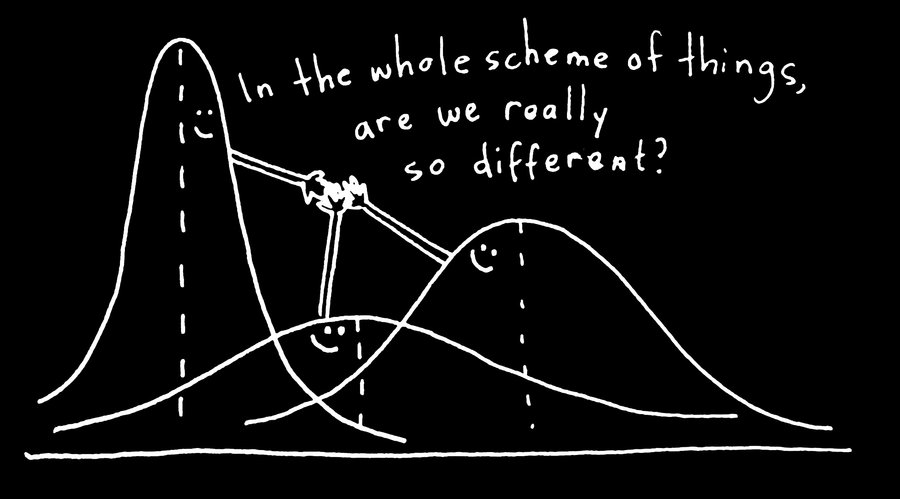
\includegraphics[scale=0.25]{ANOVA_Illustration-neg.png}
\end{frame}
%-------------- end slide -------------------------------%}}}
%-------------- start slide -------------------------------%{{{ 12.5
\begin{frame}

	\begin{enumerate}
		\item[E.g. 1] Study the relation between smoking and heart rates.\\[1em]
Generations of athletes have been cautioned that cigarette smoking impedes
performance. One measure of the truth of that warning is the effect of smoking
on heart rate. In one study, six nonsmokers, six light smokers, six moderate
smokers, and six heavy smokers each engaged in sustained physical exercise.
Table 8.1.1 lists their heart rates after they had rested for three minutes.
\\[1em]
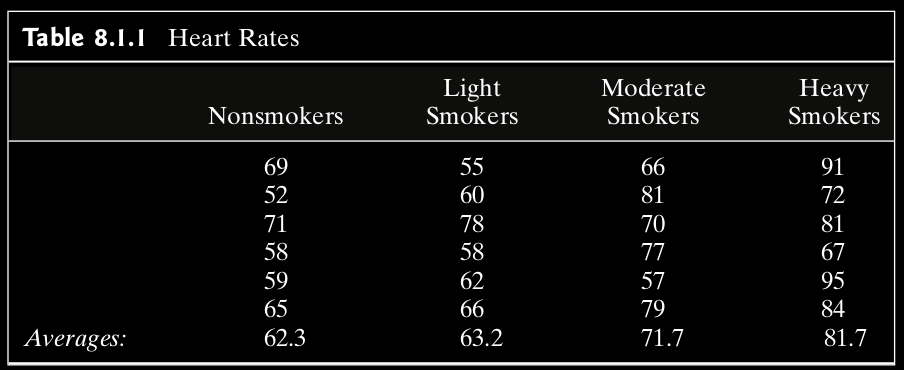
\includegraphics[scale=0.25]{Table_8-1-1-neg.png}
\item[] Show whether smoking affects heart rates at $\alpha=0.05$.
	\end{enumerate}
\end{frame}
%-------------- end slide -------------------------------%}}}
%-------------- start slide -------------------------------%{{{ 12.6
\begin{frame}
	\begin{enumerate}
		\item[E.g. 2] A certain fraction of antibiotics injected into the bloodstream are ``bound'' to
serum proteins. This phenomenon bears directly on the effectiveness of the
medication, because the binding decreases the systemic uptake of the drug.
Table below lists the binding percentages in bovine serum measured for five
widely prescribed antibiotics. Which antibiotics have similar binding
properties, and which are different? \\[1em]
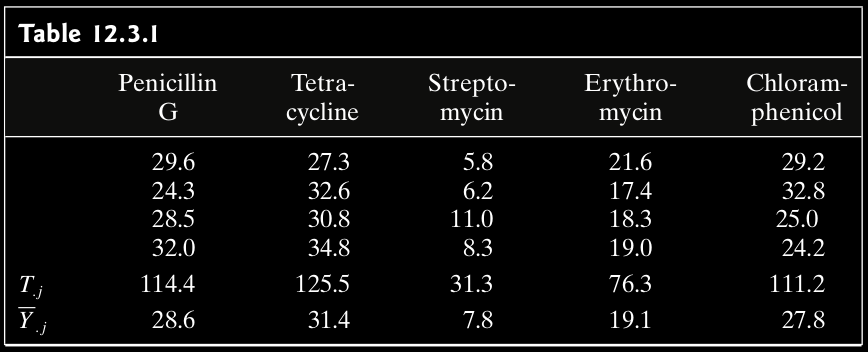
\includegraphics[scale=0.25]{Table_12-3-1-neg.png}
	\end{enumerate}
\end{frame}
%-------------- end slide -------------------------------%}}}
%-------------- start slide -------------------------------%{{{ 12.7
\begin{frame}
	\centering
	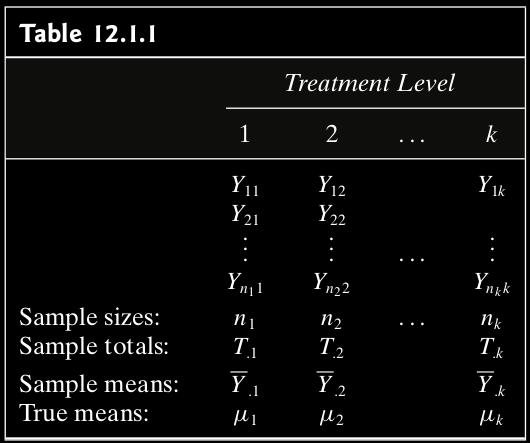
\includegraphics[scale=0.25]{Table_12-1-1-neg.png}
	\vfill
	\begin{itemize}
		\item $k$ treatment levels; $k$ independent random sample of size $n_1,\cdots, n_k$
			\vfill
		\item Total sample size: $n=\sum_{i=1}^k n_i$
			\vfill
		\item $Y_{ij}$: $i$-th observation for the $j$-th level.
			\vfill
		\item Sample total: $T_{\cdot j} = \sum_{i=1}^{n_j}Y_{i j}$
			\vfill
		\item Sample mean: $\overline{Y}_{\cdot j} = \frac{1}{n_j}\sum_{i=1}^{n_j}Y_{i j} = \frac{T_{\cdot j}}{n_j}$
			\vfill
		\item Overall total: $T_{\cdot \cdot} = \sum_{j=1}^k \sum_{i=1}^{n_j}Y_{i j}=\sum_{j=1}^k T_{\cdot j}$
			\vfill
		\item Overall mean: $\overline{Y}_{\cdot \cdot} =\frac{1}{n}\sum_{j=1}^k \sum_{i=1}^{n_j}Y_{i j} = \frac{1}{n}\sum_{j=1}^k n_j \overline{Y}_{\cdot j} = \frac{1}{n}\sum_{j=1}^k T_{\cdot j}$
	\end{itemize}
\end{frame}
%-------------- end slide -------------------------------%}}}
%-------------- start slide -------------------------------%{{{ 12.8
\begin{frame}

	\begin{enumerate}
		\item[Assume] For $j=1,\cdots, k$, $Y_{ij}\sim N(\mu_j,\sigma_j^2)$ and $\sigma_1^2 = \cdots =\sigma_k^2 = \sigma^2$ (unknown).
			\vfill
		\item[Problem] Testing
			\begin{gather*}
				H_0 : \mu_1=\mu_2=\cdots = \mu_k\\
				      \text{versus}\\
				H_1: \text{not all the $\mu_j$'s are equal}
			\end{gather*}
			\vfill
		\item[] Or testing \textcolor{yellow!80!black}{\it subhypotheses} such as\\[2em]
			\[
				H_0 : \mu_i = \mu_j \quad\text{or}\quad
				H_0 : \mu_3 = (\mu_1+\mu_2)/2
			\]
	\end{enumerate}
\end{frame}
%-------------- end slide -------------------------------%}}}
%-------------- start slide -------------------------------%{{{ 12.9
\begin{frame}
\centering
ANOVA was developed by statistician and evolutionary biologist ---
\vfill
% 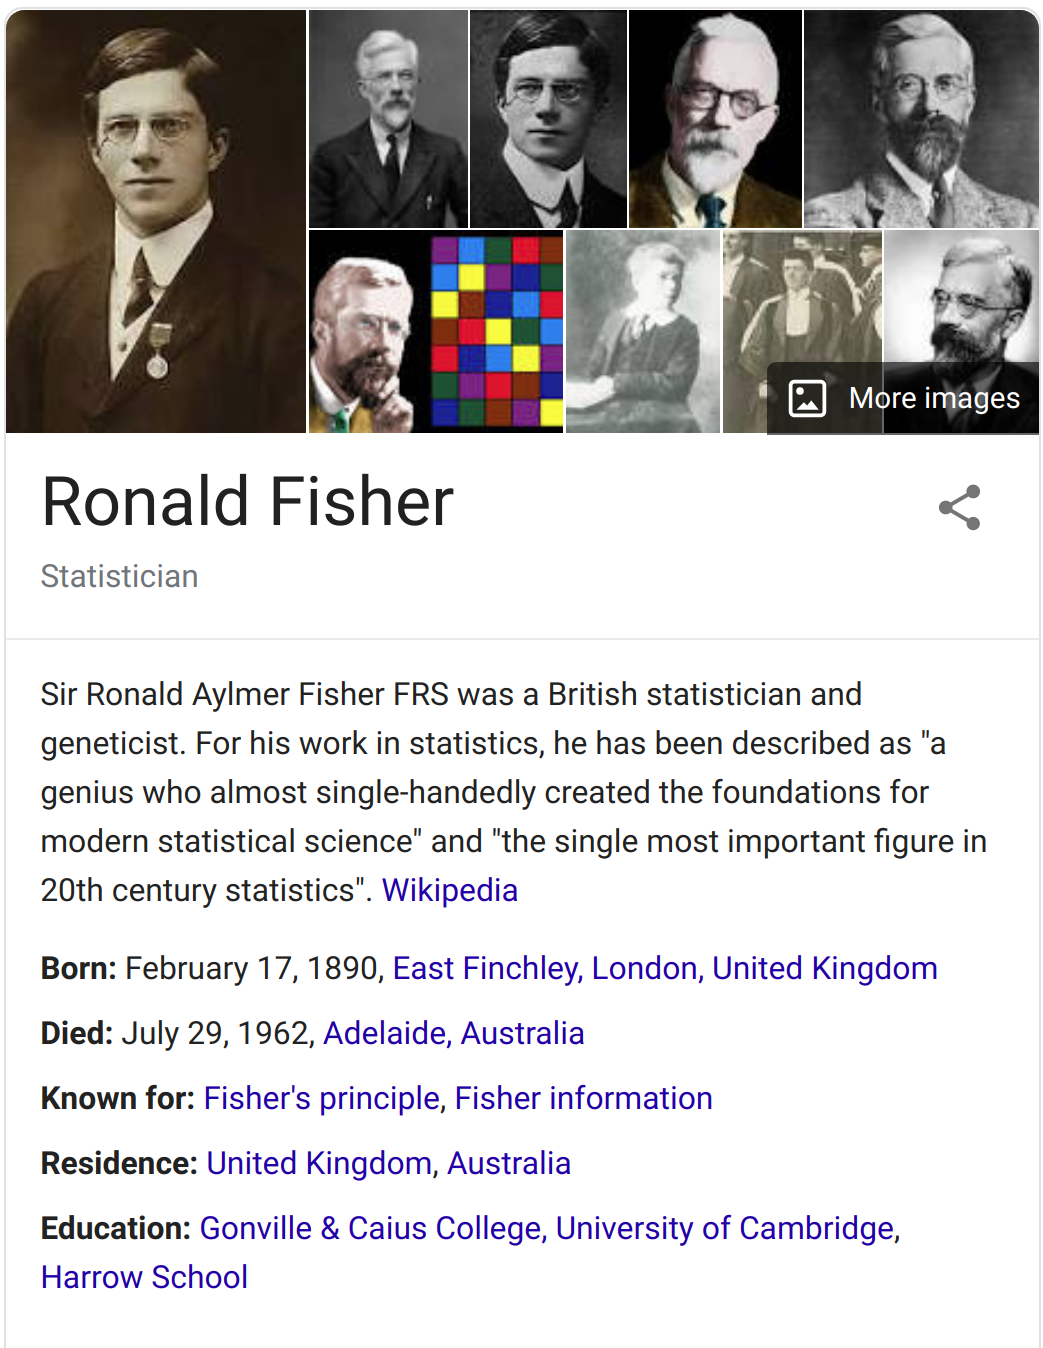
\includegraphics[scale=0.17]{Fisher.png}
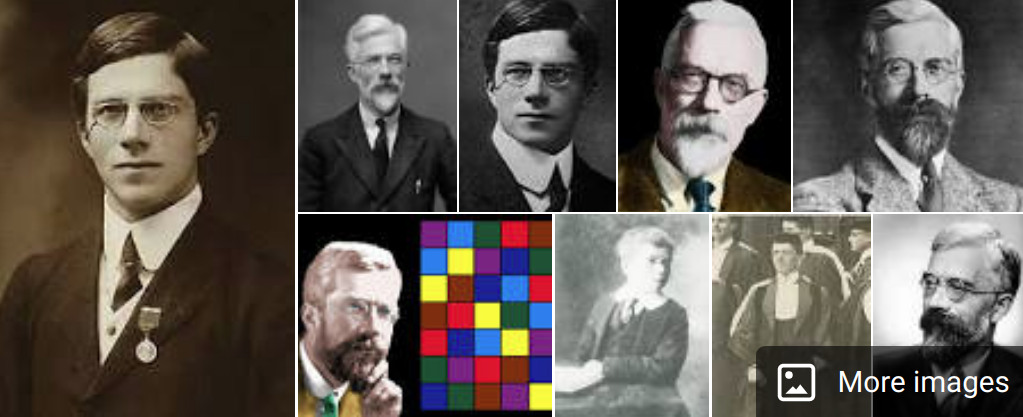
\includegraphics[scale=0.17]{Fisher-Portrait.png}
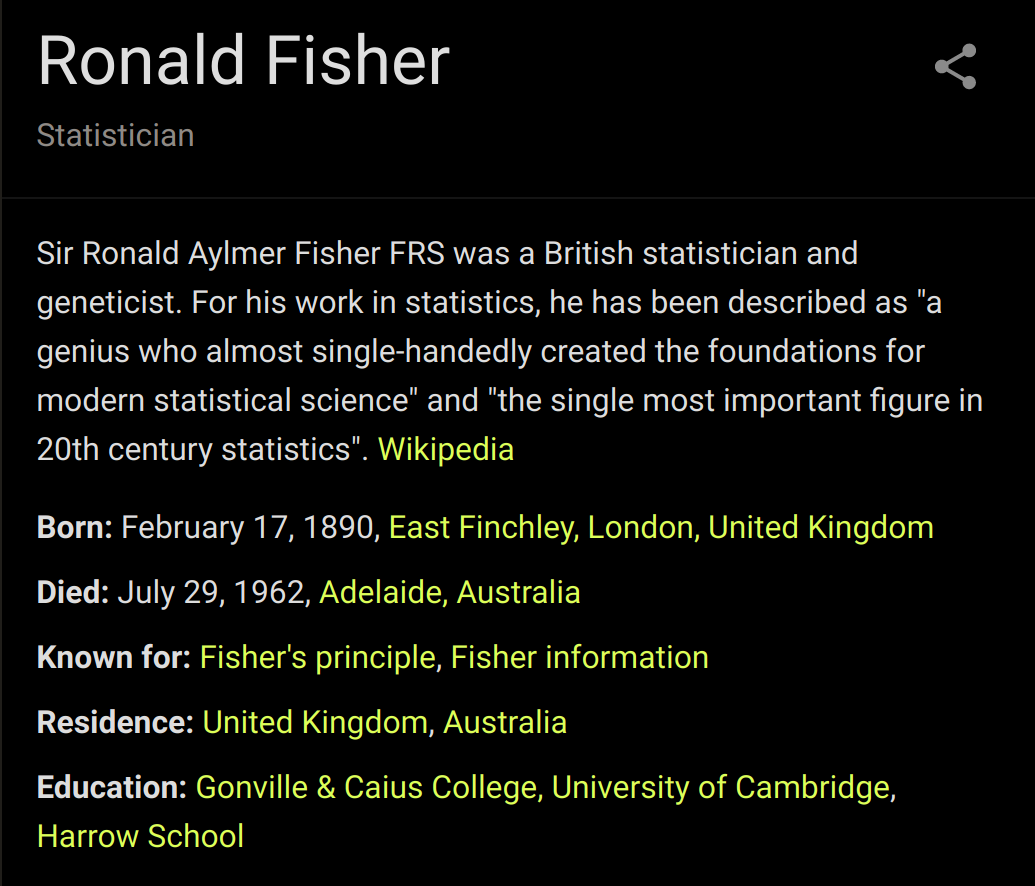
\includegraphics[scale=0.17]{Fisher-Intro-neg.png}
\end{frame}
%-------------- end slide -------------------------------%}}}
%-------------- start slide -------------------------------%{{{ 12.10
\begin{frame}[fragile]
	\begin{center}
		\url{https://www.youtube.com/watch?v=0XsovsSnRuw}
	\end{center}
\end{frame}
%-------------- end slide -------------------------------%}}}

\mySection{12.2 The $F$ Test}
%-------------- start slide -------------------------------%{{{ 12.13
\begin{frame}
	% {\S\: 12.2 The $F$ Test}
	\begin{minipage}{0.6\textwidth}
	\begin{enumerate}
		\item[] {\bf Model assumptions}
		\item Independence of observations
		\item Normality
		\item Homogeneity of variances
	\end{enumerate}
	\end{minipage}\pause
	\begin{minipage}{0.38\textwidth}
		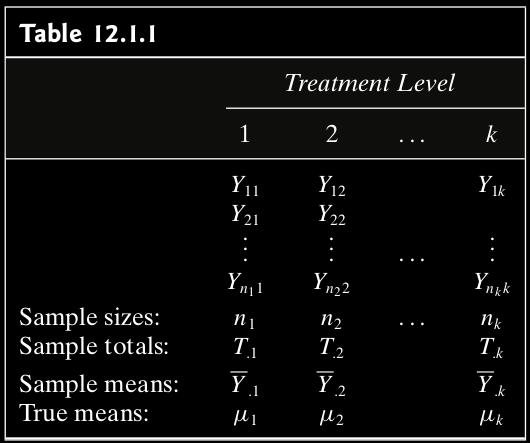
\includegraphics[scale=0.2]{Table_12-1-1-neg.png}
	\end{minipage}
\vfill

			\begin{minipage}{0.4\textwidth}
			\[\Updownarrow\]
			\end{minipage}
\vfill

	\begin{minipage}{0.4\textwidth}
		{\noindent\bf Assume:} \\
		$\forall j=1,\cdots, k$, $\forall j=1,\cdots, n_i$,
	\begin{enumerate}
		\item $Y_{ij}$ are independent.
		\item $Y_{ij}\sim N(\mu_j,\sigma^2)$
	\end{enumerate}
	\end{minipage}\pause
	\hfill $\Longleftrightarrow$ \hfill
	\begin{minipage}{0.45\textwidth}
		{\noindent\bf Assume:} \\
		$\forall j=1,\cdots, k$, $\forall j=1,\cdots, n_i$,\\
		\phantom{aaaaa} $Y_{ij} = \mu_j + \epsilon_{ij}$
	\begin{enumerate}
		\item $\epsilon_{ij}$ are independent.
		\item $\epsilon_{ij}\sim N(0,\sigma^2)$
	\end{enumerate}
	\end{minipage}
\end{frame}
%-------------- end slide -------------------------------%}}}
%-------------- start slide -------------------------------%{{{ 12.14
\begin{frame}[fragile]{Likelihood ratio test}

	\begin{enumerate}
		\item The parameter spaces are
			\[
				\Omega = \left\{
					(\mu_1,\cdots,\mu_k,\sigma^2):\:-\infty< \mu_1\alert{,\cdots,}\mu_k<\infty, \sigma^2>0
				\right\}
			\]
		\item[]
			\[
				\omega = \left\{
					(\mu_1,\cdots,\mu_k,\sigma^2):\: -\infty<\mu_1\alert{=\cdots=}\mu_k<\infty, \sigma^2>0
				\right\}
			\]
			\vfill
		\item The likelihood functions are
			\[
				L(\omega) = \left(  \frac{1}{2\pi\sigma^2}\right)^{n/2} \exp\left\{- \frac{1}{2\sigma^2}\sum_{j=1}^k\sum_{i=1}^{n_j}(y_{ij}-\alert{\mu})^2 \right\}
			\]
		\item[]
			\[
				L(\Omega) = \left(  \frac{1}{2\pi\sigma^2}\right)^{n/2} \exp\left\{- \frac{1}{2\sigma^2}\sum_{j=1}^k\sum_{i=1}^{n_j}(y_{ij}-\alert{\mu_j})^2 \right\}
			\]
	\end{enumerate}
\end{frame}
%-------------- end slide -------------------------------%}}}
%-------------- start slide -------------------------------%{{{ 12.15
\begin{frame}[fragile]

	\begin{enumerate}
		\setcounter{enumi}{2}
		\item Now
			\[
				\frac{\partial\ln L(\omega)}{\partial \mu} = \frac{1}{\sigma^2}\sum_{j=1}^k\sum_{i=1}^{n_j}(y_{ij}-\alert{\mu})
			\]
		\item[]
			\[
				\frac{\partial\ln L(\omega)}{\partial (\sigma^2)} = -\frac{n}{2\sigma^2} + \frac{1}{2\sigma^4}\sum_{j=1}^k\sum_{i=1}^{n_j}(y_{ij}-\alert{\mu})^2
			\]
			\vfill
		\item[] Setting the above derivatives to zero, the solutsions for $\mu$ and $\sigma^2$ are,
			\vfill
			\begin{align*}
				\frac 1n \sum_{j=1}^k\sum_{i=1}^{n_j} y_{ij} &= \bar{y}_{\cdot\cdot}\\
				\frac 1n \sum_{j=1}^k\sum_{i=1}^{n_j} (y_{ij}-\bar{y}_{\cdot\cdot})^2 &=v
			\end{align*}
	\end{enumerate}
\end{frame}
%-------------- end slide -------------------------------%}}}
%-------------- start slide -------------------------------%{{{ 12.16
\begin{frame}[fragile]

	\begin{enumerate}
		\item[3'] Similarly,
			\[
				\frac{\partial\ln L(\Omega)}{\partial \mu_j} = \frac{1}{\sigma^2}\sum_{j=1}^k\sum_{i=1}^{n_j}(y_{ij}-\alert{\mu_j}),\quad j=1,\cdots,k
			\]
		\item[]
			\[
				\frac{\partial\ln L(\Omega)}{\partial (\sigma^2)} = -\frac{n}{2\sigma^2} + \frac{1}{2\sigma^4}\sum_{j=1}^k\sum_{i=1}^{n_j}(y_{ij}-\alert{\mu_j})^2
			\]
			\vfill
		\item[] Setting the above derivatives to zero, the solutsions for $\mu_j$ and $\sigma^2$ are,
			\vfill
			\begin{align*}
				\frac{1}{n_j} \sum_{i=1}^{n_j} y_{ij} &= \bar{y}_{\cdot j}\\
				\frac 1n \sum_{j=1}^k\sum_{i=1}^{n_j} (y_{ij}-\bar{y}_{\cdot j})^2 &=w
			\end{align*}
	\end{enumerate}
\end{frame}
%-------------- end slide -------------------------------%}}}
%-------------- start slide -------------------------------%{{{ 12.17
\begin{frame}[fragile]

	\begin{enumerate}
		\setcounter{enumi}{3}
		\item Hence,
			\[
				L(\hat\omega)
				= \left(  \frac{n}{2\pi\sum_{j=1}^k\sum_{i=1}^{n_j}(y_{ij}-\bar{y}_{\cdot\cdot})^2}\right )^{n/2}
				\exp\left\{
					-\frac{n\sum_{j=1}^k\sum_{i=1}^{n_j}(y_{ij}-\bar{y}_{\cdot\cdot})^2}{2\sum_{j=1}^k\sum_{i=1}^{n_j}(y_{ij}-\bar{y}_{\cdot\cdot})^2}
				\right\}
			\]
		\item[]
			\[ ||\]
			\[
				\left(  \frac{n}{2\pi\sum_{j=1}^k\sum_{i=1}^{n_j}(y_{ij}-\alert{\bar{y}_{\cdot\cdot}})^2}\right )^{n/2} e^{-n/2}
			\]
			\vfill
		\item[] Similarly,
			\[
				L(\hat\Omega) =
				\left(  \frac{n}{2\pi\sum_{j=1}^k\sum_{i=1}^{n_j}(y_{ij}-\bar{y}_{\cdot j})^2}\right )^{n/2}
				\exp\left\{
					-\frac{n\sum_{j=1}^k\sum_{i=1}^{n_j}(y_{ij}-\bar{y}_{\cdot j})^2}{2\sum_{j=1}^k\sum_{i=1}^{n_j}(y_{ij}-\bar{y}_{\cdot j})^2}
				\right\}
			\]
			\[||\]
			\[
				\left(  \frac{n}{2\pi\sum_{j=1}^k\sum_{i=1}^{n_j}(y_{ij}-\alert{\bar{y}_{\cdot j}})^2}\right )^{n/2} e^{-n/2}
			\]
	\end{enumerate}
\end{frame}
%-------------- end slide -------------------------------%}}}
%-------------- start slide -------------------------------%{{{ 12.18
\begin{frame}[fragile]

	\begin{enumerate}
		\setcounter{enumi}{4}
		\item Finally,
			\vfill
			\[
				\lambda =  \frac{L(\hat\omega)}{L(\hat\Omega)} =
				\left(  \frac{\sum_{j=1}^k\sum_{i=1}^{n_j}(y_{ij}-\alert{\bar{y}_{\cdot j}})^2}{\sum_{j=1}^k\sum_{i=1}^{n_j}(y_{ij}-\alert{\bar{y}_{\cdot \cdot}})^2}\right )^{n/2}
			\]
			\vfill
		\item[$\Rightarrow$] Test statistic:
			\vfill
			\[
				\Lambda =  \frac{L(\hat\omega)}{L(\hat\Omega)} =
				\left(  \frac{\sum_{j=1}^k\sum_{i=1}^{n_j}(Y_{ij}-\alert{\bar{Y}_{\cdot j}})^2}{\sum_{j=1}^k\sum_{i=1}^{n_j}(Y_{ij}-\alert{\bar{Y}_{\cdot \cdot}})^2}\right )^{n/2}
			\]
	\end{enumerate}
\end{frame}
%-------------- end slide -------------------------------%}}}
%-------------- start slide -------------------------------%{{{ 12.19
\begin{frame}[fragile]

	\begin{enumerate}
		\item[]
	\begin{align*}
		SSTOT := & \sum_{j=1}^k\sum_{i=1}^{n_j} \left(Y_{ij}-\overline{Y}_{\cdot\cdot} \right)^2
		     \\ & =  \sum_{j=1}^k\sum_{i=1}^{n_j}\left[ \left(Y_{ij}-\overline{Y}_{\cdot j} \right)+\left(\overline{Y}_{\cdot j} - \overline{Y}_{\cdot\cdot}\right)\right]^2
		     \\ & =  \sum_{j=1}^k\sum_{i=1}^{n_j}\left(Y_{ij}-\overline{Y}_{\cdot j} \right)^2+ \text{zero cross term}+\sum_{j=1}^k\sum_{i=1}^{n_j}\left(\overline{Y}_{\cdot j} - \overline{Y}_{\cdot\cdot}\right)^2
		     \\ & =  \underbrace{\sum_{j=1}^k\sum_{i=1}^{n_j}\left(Y_{ij}-\overline{Y}_{\cdot j} \right)^2}_{\displaystyle SSE }+\underbrace{\sum_{j=1}^{k}n_j \left(\overline{Y}_{\cdot j} - \overline{Y}_{\cdot\cdot}\right)^2}_{\displaystyle SSTR}
	\end{align*}
\item[]
	\vfill
	\[\Downarrow\]
	\vfill
	\[
		\Lambda = \left(  \frac{SSE}{SSTOT}\right )^{n/2}
		= \left(  \frac{SSE}{SSE+SSTR}\right )^{n/2}
		= \left(  \frac{1}{1+SSTR/SSE}\right )^{n/2}
	\]
	\end{enumerate}
\end{frame}
%-------------- end slide -------------------------------%}}}
%-------------- start slide -------------------------------%{{{ 12.20
\begin{frame}[fragile]

	\begin{enumerate}
		\setcounter{enumi}{5}
	\item Critical regions: for some $\lambda_*\in (0,1)$ close to $0$,
		\vfill
	\item[]
			\begin{align*}
				\alpha & = \bbP \left(\Lambda \le \lambda_* \right)
				\\[1em]&=
				     \bbP \left(  \frac{1}{1+SSTR/SSE}\le \lambda_*^{2/n}\right )
				     \\[1em]&=
				     \bbP \left(   \frac{SSTR}{SSE} \le \lambda_*^{-2/n}-1\right )
				     \\[1em]&=
				     \bbP \left(   \frac{SSTR/(k-1)}{SSE/(n-k)} \le \left(\lambda_*^{-2/n}-1\right) \frac{n-k}{k-1}\right )
			\end{align*}
			\vfill
		\item We will prove that under $H_0$, $ \frac{SSTR/(k-1)}{SSE/(n-k)}\sim$ F-distr. $df_1=k-1, df_2=n-k$
			\vfill
			\[
				\Rightarrow\quad\left(\lambda_*^{-2/n}-1\right) \frac{n-k}{k-1} = F_{1-\alpha,k-1,n-k}.
			\]
			\myEnd
	\end{enumerate}
\end{frame}
%-------------- end slide -------------------------------%}}}
%-------------- start slide -------------------------------%{{{ 12.21
\begin{frame}[fragile]{Treatment sum of squares: SSTR}
	\begin{center}
		\begin{tabular}{l|cccc|c} \hline
Sample size:  & $n_1$                                                                               & $n_2$                                                                               & $\cdots$ & $n_k$                                                                               & $n=\sum_{j=1}^k n_j$                                                         \\
(Weights)     &                                                                                     &                                                                                     &          &                                                                                     &                                                                              \\
              &                                                                                     &                                                                                     &          &                                                                                     & {\it Weighted average}                                                       \\ \hline \\ [1em]
Sample means: & $\overline{Y}_{\cdot 1}$                                                            & $\overline{Y}_{\cdot 2}$                                                            & $\cdots$ & $\overline{Y}_{\cdot k}$                                                            & $\overline{Y}_{\cdot \cdot}=\frac 1n \sum_{j=1}^kn_j \overline{Y}_{\cdot j}$ \\ [2em]
True means:   & $\mu_1$                                                                             & $\mu_2$                                                                             & $\cdots$ & $\mu_k$                                                                             & $\mu=\frac 1n \sum_{j=1}^kn_j \mu_j$                                         \\ [2em]
Squares:      & $\scriptscriptstyle\left(\overline{Y}_{\cdot 1}-\overline{Y}_{\cdot\cdot}\right)^2$ & $\scriptscriptstyle\left(\overline{Y}_{\cdot 2}-\overline{Y}_{\cdot\cdot}\right)^2$ & $\cdots$ & $\scriptscriptstyle\left(\overline{Y}_{\cdot k}-\overline{Y}_{\cdot\cdot}\right)^2$ & $SSTR$
\\
\\
\hline
		\end{tabular}
	\end{center}
	\vfill
	\[
		SSTR := \sum_{j=1}^k n_j  \left(\overline{Y}_{\cdot j}-\overline{Y}_{\cdot\cdot}\right)^2
	\]
\end{frame}
%-------------- end slide -------------------------------%}}}
%-------------- start slide -------------------------------%{{{ 12.22
\begin{frame}[fragile]
	\begin{enumerate}
		\item When $k=1$, $SSTR \equiv 0$.
			\vfill
		\item When $k=2$, say $X_1,\cdots,X_n$ and $Y_1,\cdots,Y_m$:
			\[
				\overline{Y_{\cdot\cdot}} = \frac{1}{m+n} \left(n\overline{X}+m\overline{Y} \right )
			\]
			\item[]
				\begin{align*}
					SSTR & = n \left[\overline{X}-\frac{1}{n+m}\left(n\overline{X}+m \overline{Y}\right)\right]^2	+ m \left[\overline{Y}-\frac{1}{n+m}\left(n\overline{X}+m \overline{Y}\right)\right]^2 \\
               & = n\left[\frac{m(\overline{X}-\overline{Y})}{n+m}\right]^2 + m\left[\frac{n(\overline{X}-\overline{Y})}{n+m}\right]^2 \\
							 & = \left[\frac{nm^2}{(n+m)^2}+\frac{n^2m}{(n+m)^2}\right]\left(\overline{X}+\overline{Y}\right)^2\\
							 & = \frac{nm}{n+m} \left(\overline{X}-\overline{Y}\right)^2
				\end{align*}
			\item[]
			\[\]
				\[
					SSTR = \frac{\left(\overline{X}-\overline{Y}\right)^2}{\displaystyle\frac 1m + \frac 1n}
				\]
	\end{enumerate}
\end{frame}
%-------------- end slide -------------------------------%}}}
%-------------- start slide -------------------------------%{{{ 12.23
\begin{frame}[fragile]
	\begin{center}
		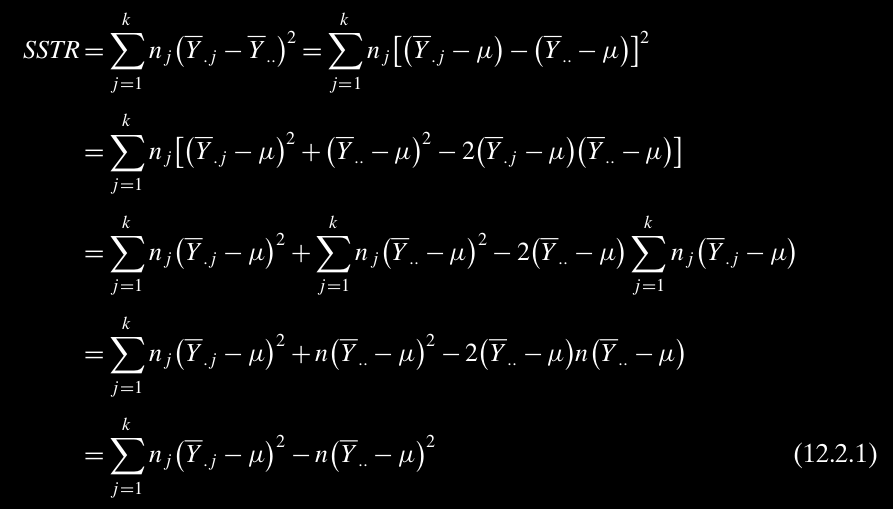
\includegraphics[scale=0.3]{Eq_12-2-1-neg.png}
	\end{center}
	\[\Downarrow\]
	\[
		SSTR = \sum_{j=1}^k n_j\left[\left(\overline{Y}_{\cdot j}-\mu_j \right)^2 - 2 \left(\overline{Y}_{\cdot j}-\mu_j \right) \left(\mu-\mu_j \right)+ \left(\mu-\mu_j \right)^2\right ]	-n  \left(\overline{Y}_{\cdot \cdot}-\mu \right)^2
	\]
\end{frame}
%-------------- end slide -------------------------------%}}}
%-------------- start slide -------------------------------%{{{ 12.24
\begin{frame}[fragile]

\begin{enumerate}
	\item[] Notice that \\[1em]
		\[
			\overline{Y}_{\cdot j}\sim N(\mu_j,\sigma^2/n_j)\qquad\text{and}\qquad
			\overline{Y}_{\cdot \cdot}\sim N(\mu,\sigma^2/n)
		\]
		\vfill
	\item[$\Longrightarrow$]
		\begin{align*}
			\E[SSTR]  =& \sum_{j=1}^k n_j \left[\frac{\sigma^2}{n_j} -2\times 0 + (\mu-\mu_j)^2\right]- n \frac{\sigma^2}{n}\\[1em]
			=& (k-1)\sigma^2 + \sum_{j=1}^k n_j (\mu-\mu_j)^2
		\end{align*}
		\vfill
	\item[Remark]
		\begin{enumerate}
			\item[] When $\mu_1=\cdots=\mu_j$ then \\[1em]
			\item $\E[SSTR]=(k-1)\sigma^2$  \\[1em]
			\item $MSTR:=\frac{SSTR}{k-1}$
				is an unbiased estimator for $\sigma^2$.\\[1em]
			\item $SSTR/\sigma^2 \sim$ Chi square $(df=k-1)$.\hfill (Homework)
		\end{enumerate}
\end{enumerate}
\end{frame}
%-------------- end slide -------------------------------%}}}
%-------------- start slide -------------------------------%{{{ 12.25
\begin{frame}[fragile]

	\begin{enumerate}
		\item[] Test $H_0:\mu_1=\cdots=\mu_k$ v.s. $\mu_j$ are not the same.
			\vfill
		\item[Case I.] when $\sigma^2$ is known.\\[2em]
		\item[] Reject $H_0$ if $SSTR/\sigma^2\ge \chi^2_{1-\alpha,k-1}$.
			\vfill
		\item[Case II.] when $\sigma^2$ is unknown.\\[2em]
		\item[] ......
	\end{enumerate}
\end{frame}
%-------------- end slide -------------------------------%}}}
%-------------- start slide -------------------------------%{{{ 12.26
\begin{frame}[fragile]{Sum of Squared Errors: SSE}

	\begin{enumerate}
		\item Sum of squred error:
			\vfill
	\begin{align*}
		SSE:=& \sum_{j=1}^k\sum_{i=1}^{n_j} \left(Y_{ij}-\overline{Y}_{\cdot j} \right)^2\\[1em]
		=& \sum_{j=1}^k(n_j-1)\left[ \frac{1}{n_j-1} \sum_{i=1}^{n_j} \left(Y_{ij}-\overline{Y}_{\cdot j} \right)^2\right]\\[1em]
		=&\sum_{j=1}^k(n_j-1) S_j^2
	\end{align*}
	\vfill
	\item Pooled variance $S_p^2$:
		\vfill
	\[
		S_p^2 = \frac{SSE}{\sum_{j=1}^k (n_j-1)} = \frac{SSE}{n-k}
	\]
\item[] Mean square of error $MSE = S_p^2$
	\end{enumerate}
\end{frame}
%-------------- end slide -------------------------------%}}}
%-------------- start slide -------------------------------%{{{ 12.27
\begin{frame}[fragile]


\begin{enumerate}
	\item[] Notice that\\[1em]
	\item $(n_j-1)S_j^2/\sigma^2\sim $Chi square $(df=n_j-1)$
	\item $S_j^2$'s are independent
	\item $SSE/\sigma^2 = (n-k) S_p^2/\sigma^2= \sum_{j=1}^k (n_j-1)S_j^2/\sigma^2 $,
	\item[] \qquad\qquad Sum of independent of Chi squares
		\[\Downarrow\]
	\item[Thm.] No mattter $H_0:\mu_1=\cdots=\mu_k$ is true or not
	\item[a.] $SSE/\sigma^2 = (n-k) S_p^2/\sigma^2\sim$ Chi square $(df=\sum_{j=1}^k(n_j-1) = n-k)$
	\item[b.] $SSTR \perp SSE$.
		\vfill
	\item[Proof.] We have shown part (a). Part (b) is trickier. Indeed, both parts are a consequence of \textcolor{yellow!80!black}{\bf Cochran's theorem}\footnote{\url{https://en.wikipedia.org/wiki/Cochran\%27s_theorem}} ... \myEnd
\end{enumerate}

\end{frame}
%-------------- end slide -------------------------------%}}}
%-------------- start slide -------------------------------%{{{ 12.28
\begin{frame}[fragile]

	\begin{enumerate}
		\item[] Let's see two special cases of
			\vfill
	\item[Thm.] No mattter $H_0:\mu_1=\cdots=\mu_k$ is true or not
	\item[a.] $SSE/\sigma^2 = (n-k) S_p^2/\sigma^2\sim$ Chi square $(df=\sum_{j=1}^k(n_j-1) = n-k)$
	\item[b.] $SSTR \perp SSE$.
		\vfill
	\item[Cases]
			\setcounter{enumi}{0}
		\item $k=1$, one sample case, $S_p^2$ is sample variance\hfill {\small Chapter 7}\\[0.6em]
		\item[] a. $(n-1)S^2/\sigma^2\sim \chi^2(n-1)$
		\item[] b. $SSTR\equiv 0$\\[1em]
		\item $k=2$, two sample case\hfill {\small Chapter 9}\\[0.6em]
		\item[] a. $(n-2)S_p^2/\sigma^2 \sim\chi^2(n-2)$
		\item[] b. $\overline{X}-\overline{Y}\perp S_p^2$ $\quad\Longleftrightarrow\quad$ $SSTR\perp SSE$
	\end{enumerate}
\end{frame}
%-------------- end slide -------------------------------%}}}
%-------------- start slide -------------------------------%{{{ 12.29
\begin{frame}[fragile]
Under $H_0: \mu_1=\cdots = \mu_k$
\begin{enumerate}
	\item $SSTR/\sigma^2 \sim \chi^2(k-1)$
	\item $SSE/\sigma^2 \sim \chi^2(n-k)$
	\item $SSTR\perp SSE$
		\vfill
	\item[$\Longrightarrow$] $\qquad \displaystyle F = \frac{SSTR/(k-1)}{SSE/(n-k)}\sim F(df_1=k-1,df_2=n-k)$
		\vfill
	\item[Reject] $H_0$ if $F\ge F_{1-\alpha,k-1,n-k}$
\end{enumerate}
\end{frame}
%-------------- end slide -------------------------------%}}}
%-------------- start slide -------------------------------%{{{ 12.30
\begin{frame}[fragile]{Total Sum of Squares: SSTOT\\[0.4em]
	SSTOT=SSE+SSTR}

	\[SSTOT:= \sum_{j=1}^k\sum_{i=1}^{n_j} \left(Y_{ij}-\overline{Y}_{\cdot \cdot} \right)^2
	\]
	\[||\]
	\begin{gather*}
		\sum_{j=1}^k\sum_{i=1}^{n_j}\left[ \left(Y_{ij}-\overline{Y}_{j \cdot} \right)+ \left(\overline{Y}_{\cdot j}-\overline{Y}_{\cdot \cdot} \right) \right]^2
 \\ ||\\
 \sum_{j=1}^k\sum_{i=1}^{n_j}\left(Y_{ij}-\overline{Y}_{j \cdot} \right)^2+2\sum_{j=1}^k\sum_{i=1}^{n_j}\left(Y_{ij}-\overline{Y}_{\cdot j} \right)\left(\overline{Y}_{\cdot j}-\overline{Y}_{\cdot \cdot} \right)+\sum_{j=1}^k\sum_{i=1}^{n_j}\left(\overline{Y}_{\cdot j}-\overline{Y}_{\cdot \cdot} \right)^2
 \\ ||\\
 \sum_{j=1}^k\sum_{i=1}^{n_j}\left(Y_{ij}-\overline{Y}_{j \cdot} \right)^2+2\sum_{j=1}^k\left(\overline{Y}_{\cdot j}-\overline{Y}_{\cdot \cdot} \right)\sum_{i=1}^{n_j}\left(Y_{ij}-\overline{Y}_{\cdot j} \right)+\sum_{j=1}^kn_j\left(\overline{Y}_{\cdot j}-\overline{Y}_{\cdot \cdot} \right)^2
 \\ ||\\
 SSE + 0 + SSTR
	\end{gather*}
\end{frame}
%-------------- end slide -------------------------------%}}}
%-------------- start slide -------------------------------%{{{ 12.31
\begin{frame}[fragile]
	\begin{center}
		\begin{tabular}{ccccc}
			$\displaystyle SSTOT$ &
			= &
			$\displaystyle SSE$ &
			+ &
			$\displaystyle SSTR$ \\ \\
			  &$\Downarrow$&&& \\ \\
			$\displaystyle \frac{SSTOT}{\sigma^2}$ &
			= &
			$\displaystyle \frac{SSE}{\sigma^2}$ &
			+ &
			$\displaystyle \frac{SSTR}{\sigma^2}$ \\ \\
			$\wr$&& $\wr$ &  & $\wr$ \\ \\
			$\chi^2(n-1)$ && $\chi^2(n-k)$ & $\perp$ & $\chi^2(k-1)$
			\\[2em]
			Under $H_0$& & \checkmark && Under $H_0$
		\end{tabular}
	\end{center}
\end{frame}
%-------------- end slide -------------------------------%}}}
%-------------- start slide -------------------------------%{{{ 12.32
\begin{frame}
	\centering
	% 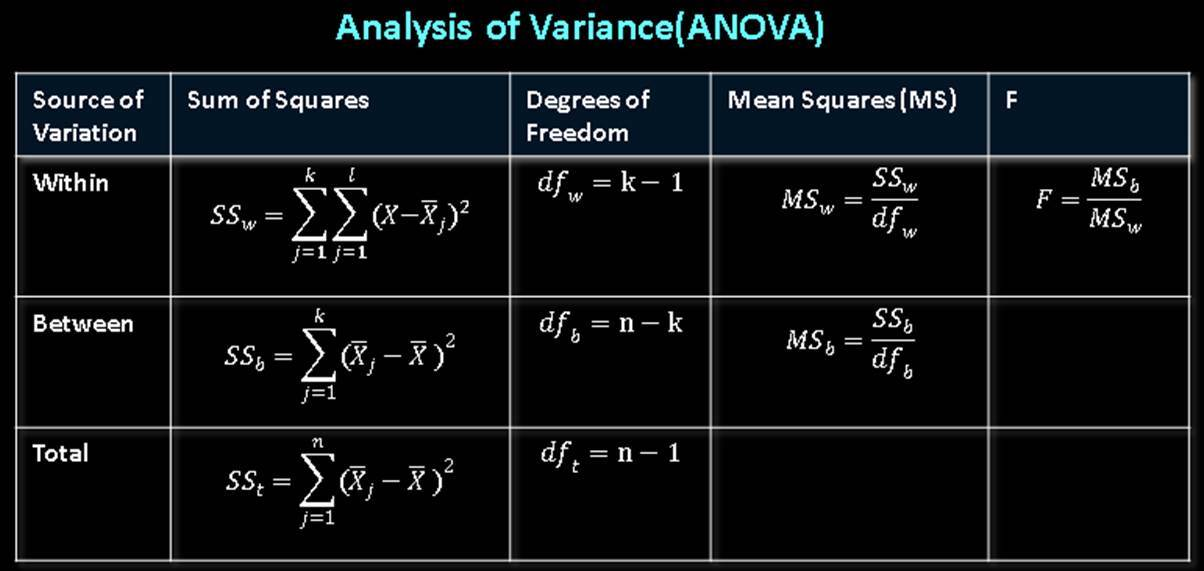
\includegraphics[scale=0.4]{Anova_Table-neg.jpg}
	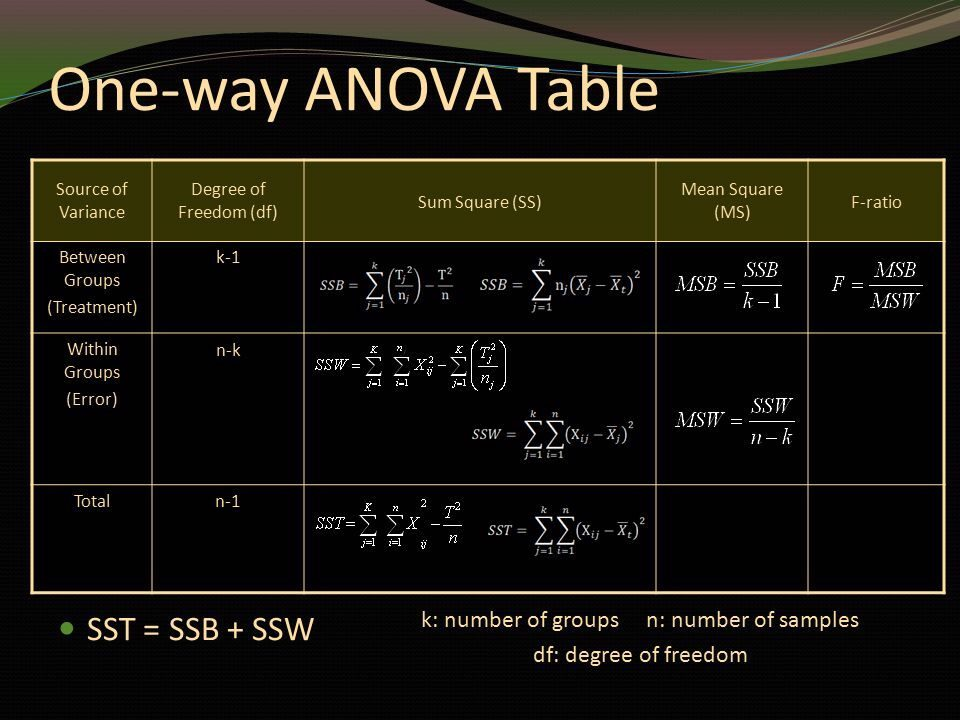
\includegraphics[scale=0.25]{Anova_Table3-neg.jpg}
	\vfill
	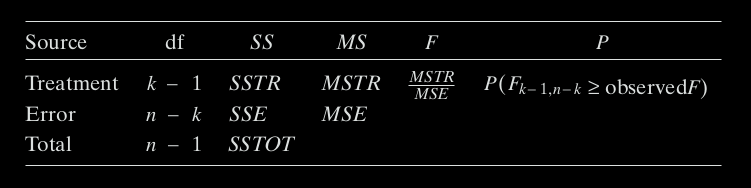
\includegraphics[scale=0.3]{Figure_12-2-1-neg.png}
\end{frame}
%-------------- end slide -------------------------------%}}}
%-------------- start slide -------------------------------%{{{ 12.33
\begin{frame}{Common notation}

\begin{enumerate}
	\item[d.f.\hspace{1.2em}]\phantom{a}\\[2em]
	\item[k-1\hspace{1.2em}]  Error sum of squares \hfill $SSE = SSW = SS_{within}$
	\item[] Mean square of error\hfill $MSE=MSW=MS_{within}=S_p^2$
	\item[] (Pooled sample variance)
		\vfill
	\item[n-k\hspace{1.2em}] Treatment sum of squares \hfill $SSTR = SSB = SS_{between}$
	\item[] Mean square of treatment\hfill $MSTR = MSB=MS_{between}$
		\vfill
	\item[n-1\hspace{1.2em}] Total sum of squares:\hfill $SST = SSTOT$
\end{enumerate}
\end{frame}
%-------------- end slide -------------------------------%}}}
%-------------- start slide -------------------------------%{{{ 12.34
\begin{frame}[fragile]{One way ANOVA v.s. Two sample $t$-test}
\begin{enumerate}
	\item[] Let $X_1,\cdots, X_n$ and $Y_1,\cdots, Y_m$ be samples from $N(\mu_X,\sigma^2)$ and $N(\mu_Y,\sigma^2)$, respectively.
		\vfill
	\item[Recall]
	\item $\displaystyle SSTR/\sigma^2 = \frac{\left(\overline{X}-\overline{Y}\right)^2}{\sigma^2\left(\frac 1n+\frac 1m\right)}\hspace{4em}\sim \chi^2(1)$
	\item $SSE/\sigma^2 = (n+m-2)S_p^2/\sigma^2\hspace{2em}\sim\chi^2(n+m-2)$
		\vfill
	\item[$\Longrightarrow$] $\displaystyle F= \frac{SSTR/1}{SSE/(n+m-2)}=\frac{\left(\overline{X}-\overline{Y}\right)^2}{S_p^2\left(\frac 1n+\frac 1m\right)} $ $\sim F(df_1=1,df_2=n+m-2)$
	\item[] \hspace{14em}$||$
	\item[] \hspace{14em}$T^2$
		\vfill
\item[$\Longrightarrow$]
		$\alpha = \bbP\left(|T|\ge t_{\alpha/2,n+m-2} \right )
		= \bbP\left(T^2\ge t_{\alpha/2,n+m-2}^2 \right )
		=  \bbP\left( F \ge F_{1-\alpha,1,n+m-2} \right)$
\item[]\phantom{a}
	\begin{center}
	Equivalent!
	\end{center}
\end{enumerate}
\end{frame}
%-------------- end slide -------------------------------%}}}
%-------------- start slide -------------------------------%{{{ 12.35
\begin{frame}
	\begin{enumerate}
		\item[E.g. 1] Study the relation between smoking and heart rates.\\[1em]
Generations of athletes have been cautioned that cigarette smoking impedes
performance. One measure of the truth of that warning is the effect of smoking
on heart rate. In one study, six nonsmokers, six light smokers, six moderate
smokers, and six heavy smokers each engaged in sustained physical exercise.
Table 8.1.1 lists their heart rates after they had rested for three minutes.
\\[1em]
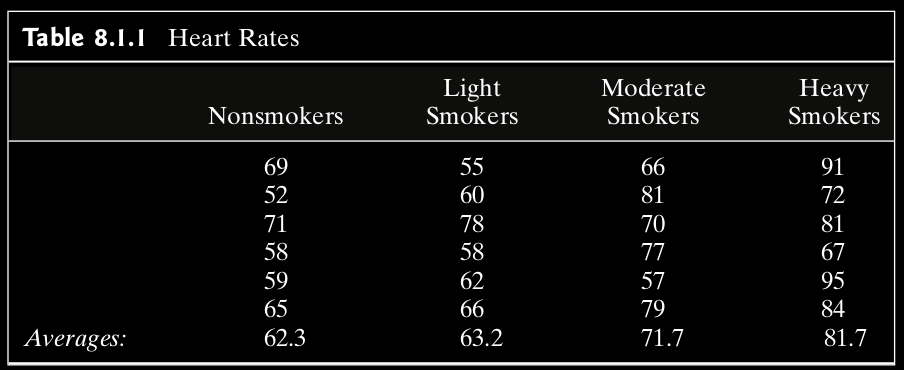
\includegraphics[scale=0.25]{Table_8-1-1-neg.png}
\item[] Show whether smoking affects heart rates at $\alpha=0.05$.
	\end{enumerate}
\end{frame}
%-------------- end slide -------------------------------%}}}
%-------------- start slide -------------------------------%{{{ 12.36
\begin{frame}

	\begin{enumerate}
		\item[Sol.] Let $\mu_1,\cdots,\mu_4$ be the true heart rates.
			\vfill
		\item[] Test $H_0:\mu_0= \cdots = \mu_4$ or not.
			\vfill
		\item[] Critical region:\\
			\vfill
			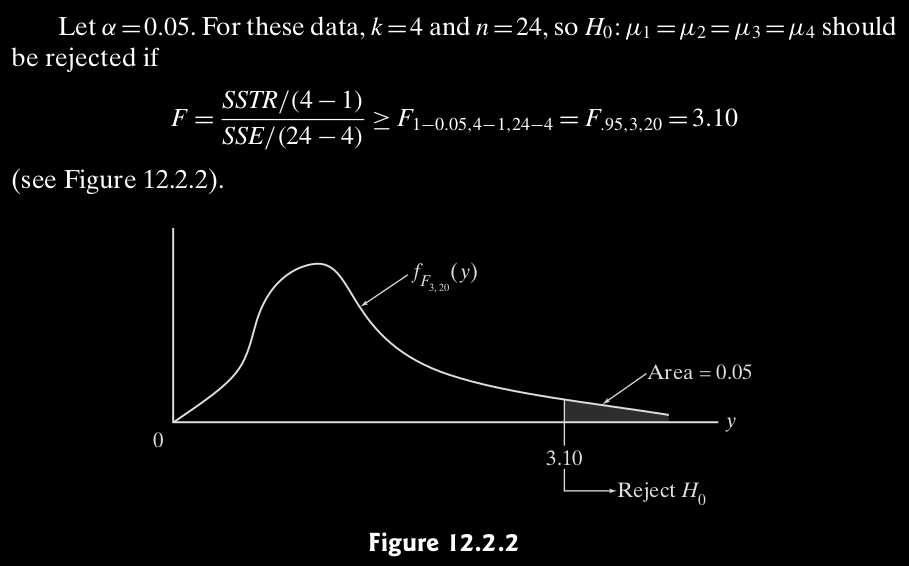
\includegraphics[scale=0.3]{Figure_12-2-2-neg.png}
	\end{enumerate}
\end{frame}
%-------------- end slide -------------------------------%}}}
%-------------- start slide -------------------------------%{{{ 12.37
\begin{frame}
\centering
	\begin{enumerate}
		\item[]  Computing....
			\vfill
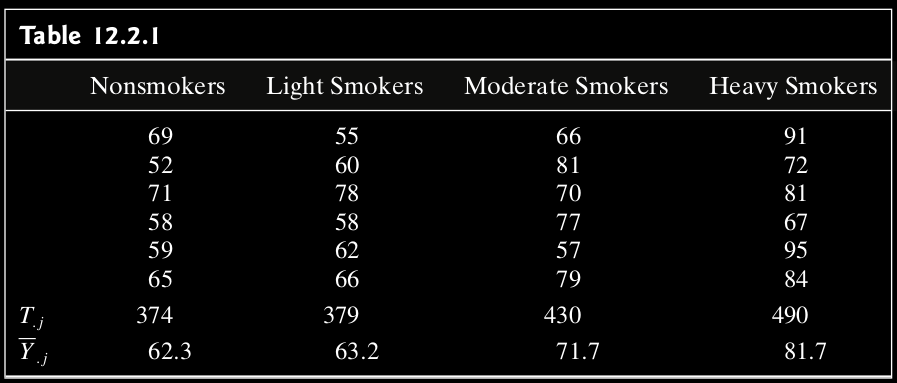
\includegraphics[scale=0.25]{Table_12-2-1-neg.png}	\\
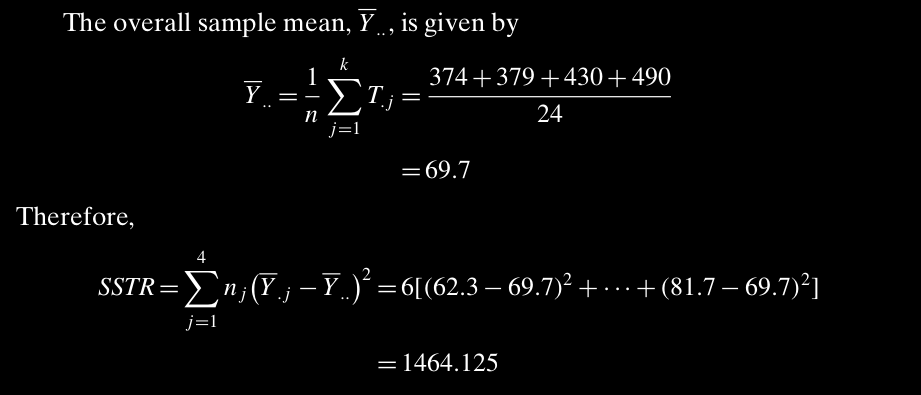
\includegraphics[scale=0.25]{Case_12-2-1-1-neg.png}\\
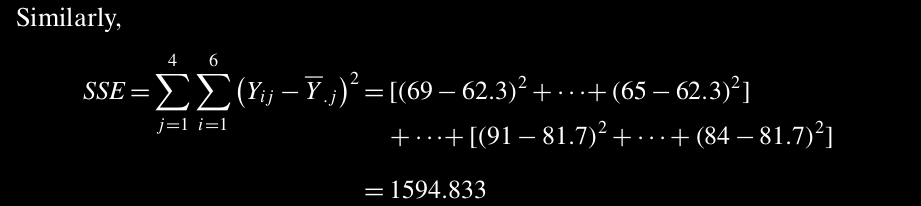
\includegraphics[scale=0.25]{Case_12-2-1-2-neg.png}
	\end{enumerate}
\end{frame}
%-------------- end slide -------------------------------%}}}
%-------------- start slide -------------------------------%{{{ 12.38
\begin{frame}
	\centering
	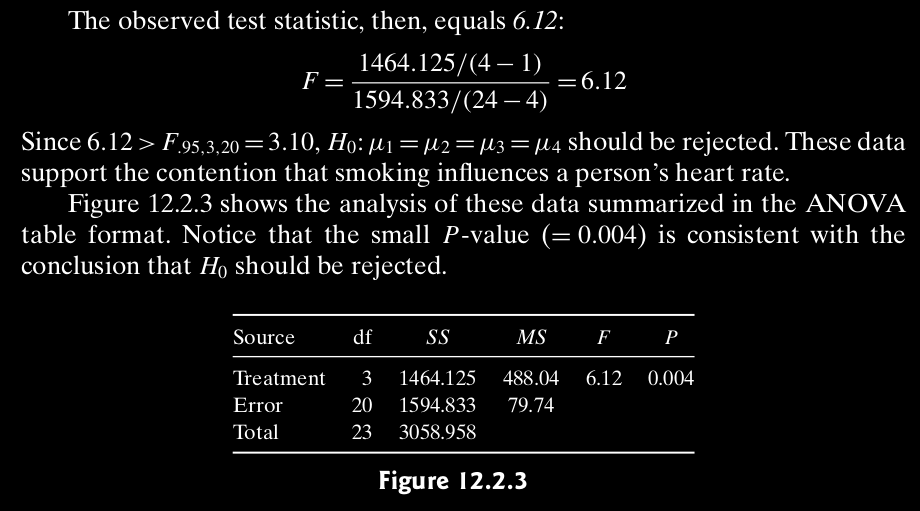
\includegraphics[scale=0.3]{Figure_12-2-3-neg.png}
	\myEnd
\end{frame}
%-------------- end slide -------------------------------%}}}
%-------------- start slide -------------------------------%{{{ 12.39
\begin{frame}[fragile]{\small\url{http://www.sthda.com/english/wiki/one-way-anova-test-in-r}}
	\begin{minipage}{0.45\textwidth}
	\begin{lstlisting}
> Input <-c("
+ rates group
+ 69  non
+ 52  non
+ 71  non
+ 58  non
+ 59  non
+ 65  non
+ 55  light
+ 60  light
+ 78  light
+ 58  light
+ 62  light
+ 66  light
+ 66  moderate
+ 81  moderate
+ 70  moderate
+ 77  moderate
+ 57  moderate
+ 79  moderate
+ 91  heavy
+ 72  heavy
+ 81  heavy
+ 67  heavy
+ 95  heavy
+ 84  heavy
+ ")
> Data = read.table(textConnection(Input),
+                   header=TRUE)
	\end{lstlisting}
	\end{minipage}
	\hfill
	\begin{minipage}{0.45\textwidth}
	\begin{lstlisting}
> Data
   rates    group
1     69      non
2     52      non
3     71      non
4     58      non
5     59      non
6     65      non
7     55    light
8     60    light
9     78    light
10    58    light
11    62    light
12    66    light
13    66 moderate
14    81 moderate
15    70 moderate
16    77 moderate
17    57 moderate
18    79 moderate
19    91    heavy
20    72    heavy
21    81    heavy
22    67    heavy
23    95    heavy
24    84    heavy
	\end{lstlisting}
	\end{minipage}
\end{frame}
%-------------- end slide -------------------------------%}}}
%-------------- start slide -------------------------------%{{{ 12.40
\begin{frame}[fragile]
	\begin{center}
	\begin{lstlisting}
> # Check the levels
> levels(Data$group)
[1] "heavy"    "light"    "moderate" "non"
> # Order the groups
> Data$group <- ordered(Data$group, levels = c("non", "light","moderate", "heavy"))
> levels(Data$group)
[1] "non"      "light"    "moderate" "heavy"
	\end{lstlisting}
	\vfill
	\begin{lstlisting}
> # Compute summary statistics by groups
> # including count, mean, sd:
> library(dplyr) # a grammar of data manipulation
> group_by(Data, group) %>%
+   summarise(
+     count = n(),
+     mean = mean(rates, na.rm = TRUE),
+     sd = sd(rates, na.rm = TRUE)
+   )
# A tibble: 4 x 4
  group    count  mean    sd
  <ord>    <int> <dbl> <dbl>
1 non          6  62.3  7.26
2 light        6  63.2  8.16
3 moderate     6  71.7  9.16
4 heavy        6  81.7 10.8
	\end{lstlisting}
	\end{center}
\end{frame}
%-------------- end slide -------------------------------%}}}
%-------------- start slide -------------------------------%{{{ 12.41
\begin{frame}[fragile]
	\begin{center}
	\begin{lstlisting}
# Box plots
# ++++++++++++++++++++
# Plot rates by group and color by group
library(ggpubr)
png("Case_12-2-1-ggboxplot.png")
ggboxplot(Data, x = "group", y = "rates",
          color = "group", palette = c("#00AFBB", "#E7B800", "#FC4E07", "blue"),
          order = c("non", "light", "moderate","heavy"),
          ylab = "Rates", xlab = "Treatment")
dev.off()
	\end{lstlisting}
	\vfill
	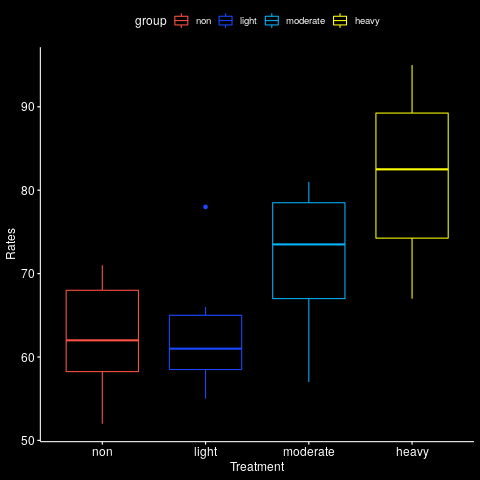
\includegraphics[scale=0.25]{Case_12-2-1-ggboxplot-neg.png}
	\end{center}
\end{frame}
%-------------- end slide -------------------------------%}}}
%-------------- start slide -------------------------------%{{{ 12.42
\begin{frame}[fragile]
	\begin{center}
	\begin{lstlisting}
# Mean plots
# ++++++++++++++++++++
# Plot rates by group
# Add error bars: mean_se
# (other values include: mean_sd, mean_ci, median_iqr, ....)
png("Case_12-2-1-ggline.png")
library(ggpubr)
ggline(Data, x = "group", y = "rates",
       add = c("mean_se", "jitter"),
       order =  c("non", "light", "moderate","heavy"),
       ylab = "Rates", xlab = "Treatment")
dev.off()
	\end{lstlisting}
	\vfill
	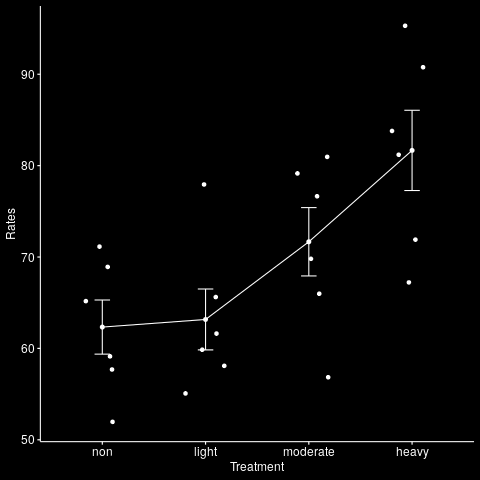
\includegraphics[scale=0.25]{Case_12-2-1-ggline-neg.png}
	\end{center}
\end{frame}
%-------------- end slide -------------------------------%}}}
%-------------- start slide -------------------------------%{{{ 12.43
\begin{frame}[fragile]
\begin{lstlisting}
> # Compute the analysis of variance
> res.aov <- aov(rates ~ group, data = Data)
> # Summary of the analysis
> summary(res.aov)
            Df Sum Sq Mean Sq F value  Pr(>F)
group        3   1464   488.0    6.12 0.00398 **
Residuals   20   1595    79.7
---
Signif. codes:  0 '***' 0.001 '**' 0.01 '*' 0.05 '.' 0.1 ' ' 1
\end{lstlisting}
\end{frame}
%-------------- end slide -------------------------------%}}}
%-------------- start slide -------------------------------%{{{ 12.44
\begin{frame}[fragile]
\begin{lstlisting}
> # Tukey multiple multiple-comparisons
> TukeyHSD(res.aov)
  Tukey multiple comparisons of means
    95% family-wise confidence level

Fit: aov(formula = rates ~ group, data = Data)

$group
                     diff        lwr      upr     p adj
light-non       0.8333333 -13.596955 15.26362 0.9984448
moderate-non    9.3333333  -5.096955 23.76362 0.2978123
heavy-non      19.3333333   4.903045 33.76362 0.0063659
moderate-light  8.5000000  -5.930289 22.93029 0.3755571
heavy-light    18.5000000   4.069711 32.93029 0.0091463
heavy-moderate 10.0000000  -4.430289 24.43029 0.2438158
\end{lstlisting}
\vfill
\begin{enumerate}
	\item diff: difference between means of the two groups
	\item lwr, upr: the lower and the upper end point of the C.I. at 95\% (default)
	\item p adj: p-value after adjustment for the multiple comparisons
		\vspace{1em}
	\item[]
		\begin{center}
			Inferences \\
		if p-value $\le 0.05$  $\quad\Longleftrightarrow\quad$ if zero is in the C.I.
		\end{center}
\end{enumerate}
\end{frame}
%-------------- end slide -------------------------------%}}}
%-------------- start slide -------------------------------%{{{ 12.45
\begin{frame}[fragile]
\begin{lstlisting}
> # Or one may use multcomp package or multiple comparisons
> library(multcomp)
> summary(glht(res.aov, linfct = mcp(group = "Tukey")))

	 Simultaneous Tests for General Linear Hypotheses

Multiple Comparisons of Means: Tukey Contrasts


Fit: aov(formula = rates ~ group, data = Data)

Linear Hypotheses:
                      Estimate Std. Error t value Pr(>|t|)
light - non == 0        0.8333     5.1556   0.162  0.99844
moderate - non == 0     9.3333     5.1556   1.810  0.29776
heavy - non == 0       19.3333     5.1556   3.750  0.00629 **
moderate - light == 0   8.5000     5.1556   1.649  0.37544
heavy - light == 0     18.5000     5.1556   3.588  0.00901 **
heavy - moderate == 0  10.0000     5.1556   1.940  0.24382
---
Signif. codes:  0 '***' 0.001 '**' 0.01 '*' 0.05 '.' 0.1 ' ' 1
(Adjusted p values reported -- single-step method)
\end{lstlisting}
\end{frame}
%-------------- end slide -------------------------------%}}}
%-------------- start slide -------------------------------%{{{ 12.46
\begin{frame}[fragile]
\begin{center}
\begin{lstlisting}
# Check ANOVA assumptions: test validity?
# diagnostic plots
layout(matrix(c(1,2),1,2)) # optional 1x2 graphs/page
plot(res.aov,c(1,2))
\end{lstlisting}
\vfill
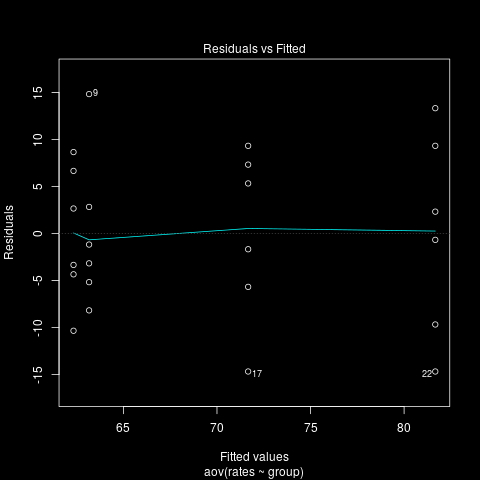
\includegraphics[scale=0.3]{Case_12-2-1-diagnostic_plots1-neg.png}
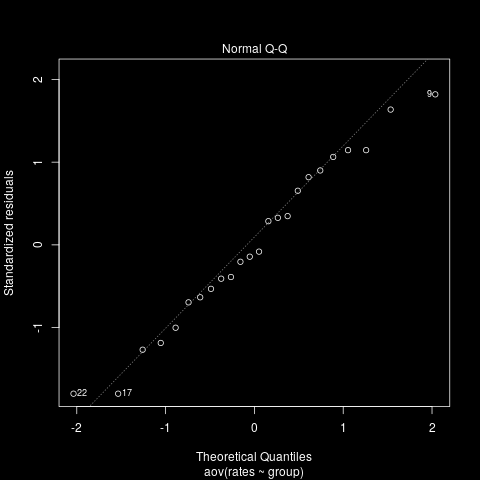
\includegraphics[scale=0.3]{Case_12-2-1-diagnostic_plots2-neg.png}
\end{center}
\end{frame}
%-------------- end slide -------------------------------%}}}
%-------------- start slide -------------------------------%{{{ 12.47
\begin{frame}[fragile]

	\begin{enumerate}
		\item Residuals vs Fitted: test homogeneity of variances\\
			One can also use Levene's test for this purpose:
		\item[]
			\begin{minipage}{0.7\textwidth}
\begin{lstlisting}
> # Use Levene's test to gest homogeneity of variances
> library(car)
> leveneTest(rates ~ group, data = Data)
Levene's Test for Homogeneity of Variance (center = median)
      Df F value Pr(>F)
group  3  0.3885 0.7625
      20
\end{lstlisting}
			\end{minipage}
\vfill
\item Normal Q-Q plot: Test normality. (It should be close to diagonal line.)\\
One can also use Shapiro-Wilk test:
\item[]
	\begin{minipage}{0.70\textwidth}
\begin{lstlisting}
# Extract the residuals
> aov_residuals <- residuals(object = res.aov )
> # Run Shapiro-Wilk test
> shapiro.test(x = aov_residuals )

	Shapiro-Wilk normality test

data:  aov_residuals
W = 0.9741, p-value = 0.7677
\end{lstlisting}
	\end{minipage}
	\end{enumerate}
\end{frame}
%-------------- end slide -------------------------------%}}}
%-------------- start slide -------------------------------%{{{ 12.48
\begin{frame}[fragile]{Non-parametric alternative to one-way ANOVA test}
	\begin{center}
	\begin{minipage}{0.7\textwidth}
\begin{lstlisting}
> # Non-parametric alternative to one-way ANOVA test
> # a non-parametric alternative to one-way ANOVA
> # is Kruskal-Wallis rank sum test, which can be
> # used when ANNOVA assumptions are not met.
> kruskal.test(rates ~ group, data = Data)

	Kruskal-Wallis rank sum test

data:  rates by group
Kruskal-Wallis chi-squared = 10.729, df = 3, p-value = 0.01329
\end{lstlisting}
	\end{minipage}
\vfill
{\small
	See Section 4 of Chapter 14 for more details.}
\end{center}
\end{frame}
%-------------- end slide -------------------------------%}}}

\mySection{12.3 Multiple Comparisons: Turkey's Method}
%-------------- start slide -------------------------------%{{{ 12.51
\begin{frame}
	% {\S\: 12.3 Multiple Comparisons: Turkey's Method}
\begin{center}
	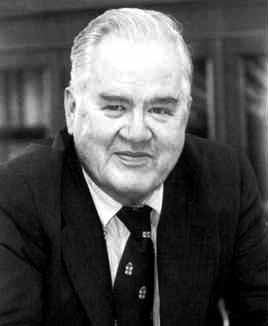
\includegraphics[scale=0.25]{John_Tukey.jpg} \\[2em]
	\small
	\begin{enumerate}
	\item John Wilder Tukey (June 16, 1915 -- July 26, 2000)
		was an American mathematician best known for
		development of the Fast Fourier Transform (FFT) algorithm and box plot.
	\item The Tukey range test, the Tukey lambda distribution,
		the Tukey test of additivity,
		and the Teichm\"uller-Tukey lemma all bear his name.
	\item  He is also credited with coining the term 'bit'.
	\end{enumerate}
	\vfill
	\url{https://en.wikipedia.org/wiki/John_Tukey}
	\end{center}
\end{frame}
%-------------- end slide -------------------------------%}}}
%-------------- start slide -------------------------------%{{{ 12.52
\begin{frame}[fragile]

	\begin{enumerate}
		\item[]
	\begin{center}
		\begin{tabular}{cccc}
			$N(\mu_1,\sigma^2)$ & $N(\mu_2,\sigma^2)$ & $\cdots$ & $N(\mu_2,\sigma^2)$ \\
			\hline
			$Y_{11}$ & $Y_{12}$ & $\cdots$ & $Y_{1k}$\cr
			$Y_{21}$ & $Y_{22}$ & $\cdots$ & $Y_{2k}$\cr
			$\vdots$ & $\vdots$ & $\vdots$ & $\vdots$\cr
			$Y_{r1}$ & $Y_{r2}$ & $\cdots$ & $Y_{rk}$\cr
			\hline
		\end{tabular}
	\end{center}
	\vfill
\item[Goal] For any $i\ne j$, test
	\[
	H_0: \mu_i =\mu_j \qquad v.s. \qquad H_1: \mu_i\ne \mu_j
	\]
	\vfill
\item[] at the $\alpha$ level of significance defined as
	\[
		\bbP \left(\bigcup_{j=1}^{{k\choose 2}}E_j\right) = \alpha
	\]
\item[] where there are ${k\choose 2}$ pairs, and $E_j$ is the event of making a type I error for the $j$-th pair.
	\end{enumerate}

\end{frame}
%-------------- end slide -------------------------------%}}}
%-------------- start slide -------------------------------%{{{ 12.53
\begin{frame}[fragile]
\begin{enumerate}
	\item[Goal'] Simultaneous C.I.'s for ${k\choose 2}$ pairs of means:
	\item[] Given $\alpha$, find $I_{ij}$, the C.I. for $\mu_i-\mu_j$ (with $i,j=1,\cdots,k$ and $i\ne j$), s.t.
	\item[]
		\[
			\bbP\left(\mu_i-\mu_j\in I_{ij},\: \forall i,j=1,\cdots, k, i\ne j\right) = 1-\alpha.
		\]
\end{enumerate}

\end{frame}
%-------------- end slide -------------------------------%}}}
%-------------- start slide -------------------------------%{{{ 12.54
\begin{frame}[fragile]

	\begin{enumerate}
		\item[???] Why not the standard pair-wise two-sample t-test?
		\item[] Suppose $\bbP(E_j)=\alpha_*$. Then
			\begin{align*}
\alpha & = \bbP \left(\bigcup_{j=1}^{{k\choose 2}}E_j\right)
= 1-  \bbP \left(\bigcap_{j=1}^{{k\choose 2}}E_j^c \right)
\approx 1- \prod_{j=1}^{k\choose 2} \bbP(E_j^c)
= 1-(1-\alpha_*)^{k\choose 2}
			\end{align*}
		\item[] Hence,
		\[
			\alpha_* \approx  1-(1-\alpha)^{1/{k\choose 2}}
		\]
		\vfill
	\item[] E.g., $\alpha=0.05$
		\begin{center}
			\begin{tabular}{c|ccc}
				$k$ & 5 & 8 & 100 \\
				\hline
				$\alpha_*$ & 0.0051162 & 0.001830 & 0.00001036
			\end{tabular}
		\end{center}
	\end{enumerate}
\end{frame}
%-------------- end slide -------------------------------%}}}
%-------------- start slide -------------------------------%{{{ 12.55
\begin{frame}[fragile]{Bonferroni's method \\
		\small --- A straightforward method}
		\begin{minipage}{0.4\textwidth}
	\begin{enumerate}
		\item[]
			\begin{align*}
				\bbP\left(\mu_i-\mu_j\in I_{ij},\: \forall i\ne j\right)
			\end{align*}
		\item[]
			\[||\]
			\[
			\bbP\left(\bigcap_{i\ne j}\mu_i-\mu_j\in I_{ij}\right)
			\]
		\item[]
			\[||\]
			\[
				1-\bbP\left(\bigcup_{i\ne j}\mu_i-\mu_j\not\in I_{ij}\right)
			\]
		\item[]
			\[\text{\rotatebox[origin=c]{90}{$\le$}}\]
			\[
				1-\sum_{i\ne j} \bbP\left(\mu_i-\mu_j\not\in I_{ij}\right)
			\]
		\item[]
			\[||\]
			\[
				1 - {k\choose 2} \alpha_*
			\]
	\end{enumerate}
		\end{minipage}
		\hfill\pause
		\begin{minipage}{0.55\textwidth}
			\begin{enumerate}
				\item
			 If we choose $\alpha_* = \alpha/{k\choose 2}$,
		 \item let $I_{ij}$ be the $(1-\alpha_*)100\%$ C.I. $i\ne j$
		 \item[]
			 \[\Downarrow\]
			\begin{align*}
				\bbP\left(\mu_i-\mu_j\in I_{ij},\: \forall i\ne j\right)
			\end{align*}
			\[\text{\rotatebox[origin=c]{90}{$\le$}}\]
			\[
				1 - {k\choose 2} \alpha_*
			\]
			\[||\]
			\[
			1-\alpha.
			\]
			\end{enumerate}
		\end{minipage}
\end{frame}
%-------------- end slide -------------------------------%}}}
%-------------- start slide -------------------------------%{{{ 12.56
\begin{frame}[fragile]

	\begin{enumerate}
\item[Remark] This is an approximation. The resulting C.I. are in general too wide.\\[1em]
\item[] The exact, and much more precise, solution is given by J.W. Turkey.\\[1em]
\item[] One can also construct simultaneous C.I. for all possible linear combinations of the parameters $\sum_{j=1}^k c_j \mu_j$, this can be acchieved by {\bf Scheff\'e's method}. A simple verson is given in \S 12.4.
	\end{enumerate}
\end{frame}
%-------------- end slide -------------------------------%}}}
%-------------- start slide -------------------------------%{{{ 12.57
\begin{frame}[fragile]{Tukey's HSD (honestly significant difference) test}
	\begin{enumerate}
		\item[] Let's construct $(1-\alpha)100\%$ C.I.'s simultaneously for all pairs.
			\vfill
		\item[]
			\[
				\bbP\left(\left|(\overline{Y}_{\cdot i}-\mu_i) - (\overline{Y}_{\cdot j}-\mu_j)\right|\le \mathcal{E},\quad \forall i\ne j\right) = 1-\alpha
			\]
		\item[]
			\[
				||
			\]
			\[
				\bbP\left(\max_{i}(\overline{Y}_{\cdot i}-\mu_i) - \min_{j}(\overline{Y}_{\cdot j}-\mu_j)\le \mathcal{E}\right)\hspace{3em}
			\]
		\item[]
			\[
				||
			\]
			\[
				\bbP\left(\max_{i}\overline{Y}_{\cdot i} - \min_{j}\overline{Y}_{\cdot j}\le \mathcal{E}\right)\hspace{3em}
			\]
			\vfill
		\item[$\Longrightarrow$]  Needs to study  ...
	\end{enumerate}
\end{frame}
%-------------- end slide -------------------------------%}}}
%-------------- start slide -------------------------------%{{{ 12.58
\begin{frame}[fragile]

	\begin{enumerate}
		\item[Def.] Let $W_1,\cdots, W_k$ be $k$ i.i.d. r.v.'s from $N(\mu,\sigma^2)$. Let $R$ denote their range:
		\[
		R =\max_i W_ i -\min_i W_i.
		\]
		Let $S^2$ be an unbiased estimator for $\sigma^2$ independent of the $W_i$'s and based on $\nu$ df.
		Define the {\bf Studentized range, $Q_{k,\nu}$}, to be the ratio:
		\[
			Q_{k,\nu} :=\frac RS.
		\]
		\vfill
	\item[]
		\begin{center}
			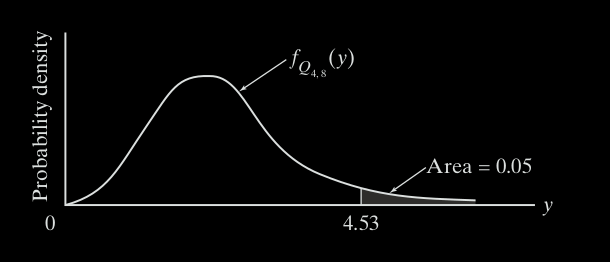
\includegraphics[scale=0.35]{Figure_12-3-1-neg.png}
		\end{center}
	\item[Remark]
		\begin{enumerate}
			\item We need $R\perp S$ to mimic Student's t-distribution.
			\item In the following $\nu = n-k = rk -k = r(k-1)$.
		\end{enumerate}
\end{enumerate}
\end{frame}
%-------------- end slide -------------------------------%}}}
%-------------- start slide -------------------------------%{{{ 12.59
\begin{frame}[fragile]
	\begin{center}

		\begin{enumerate}
			\item[] $Q_{k,\nu}\sim$ {\bf Studentized range distribution} with parameters $k$ and $\nu$.
			\item[] $k$: number of groups.
			\item[] $\nu$: degrees of freedom.
				\vfill
			\item[]
		\end{enumerate}
		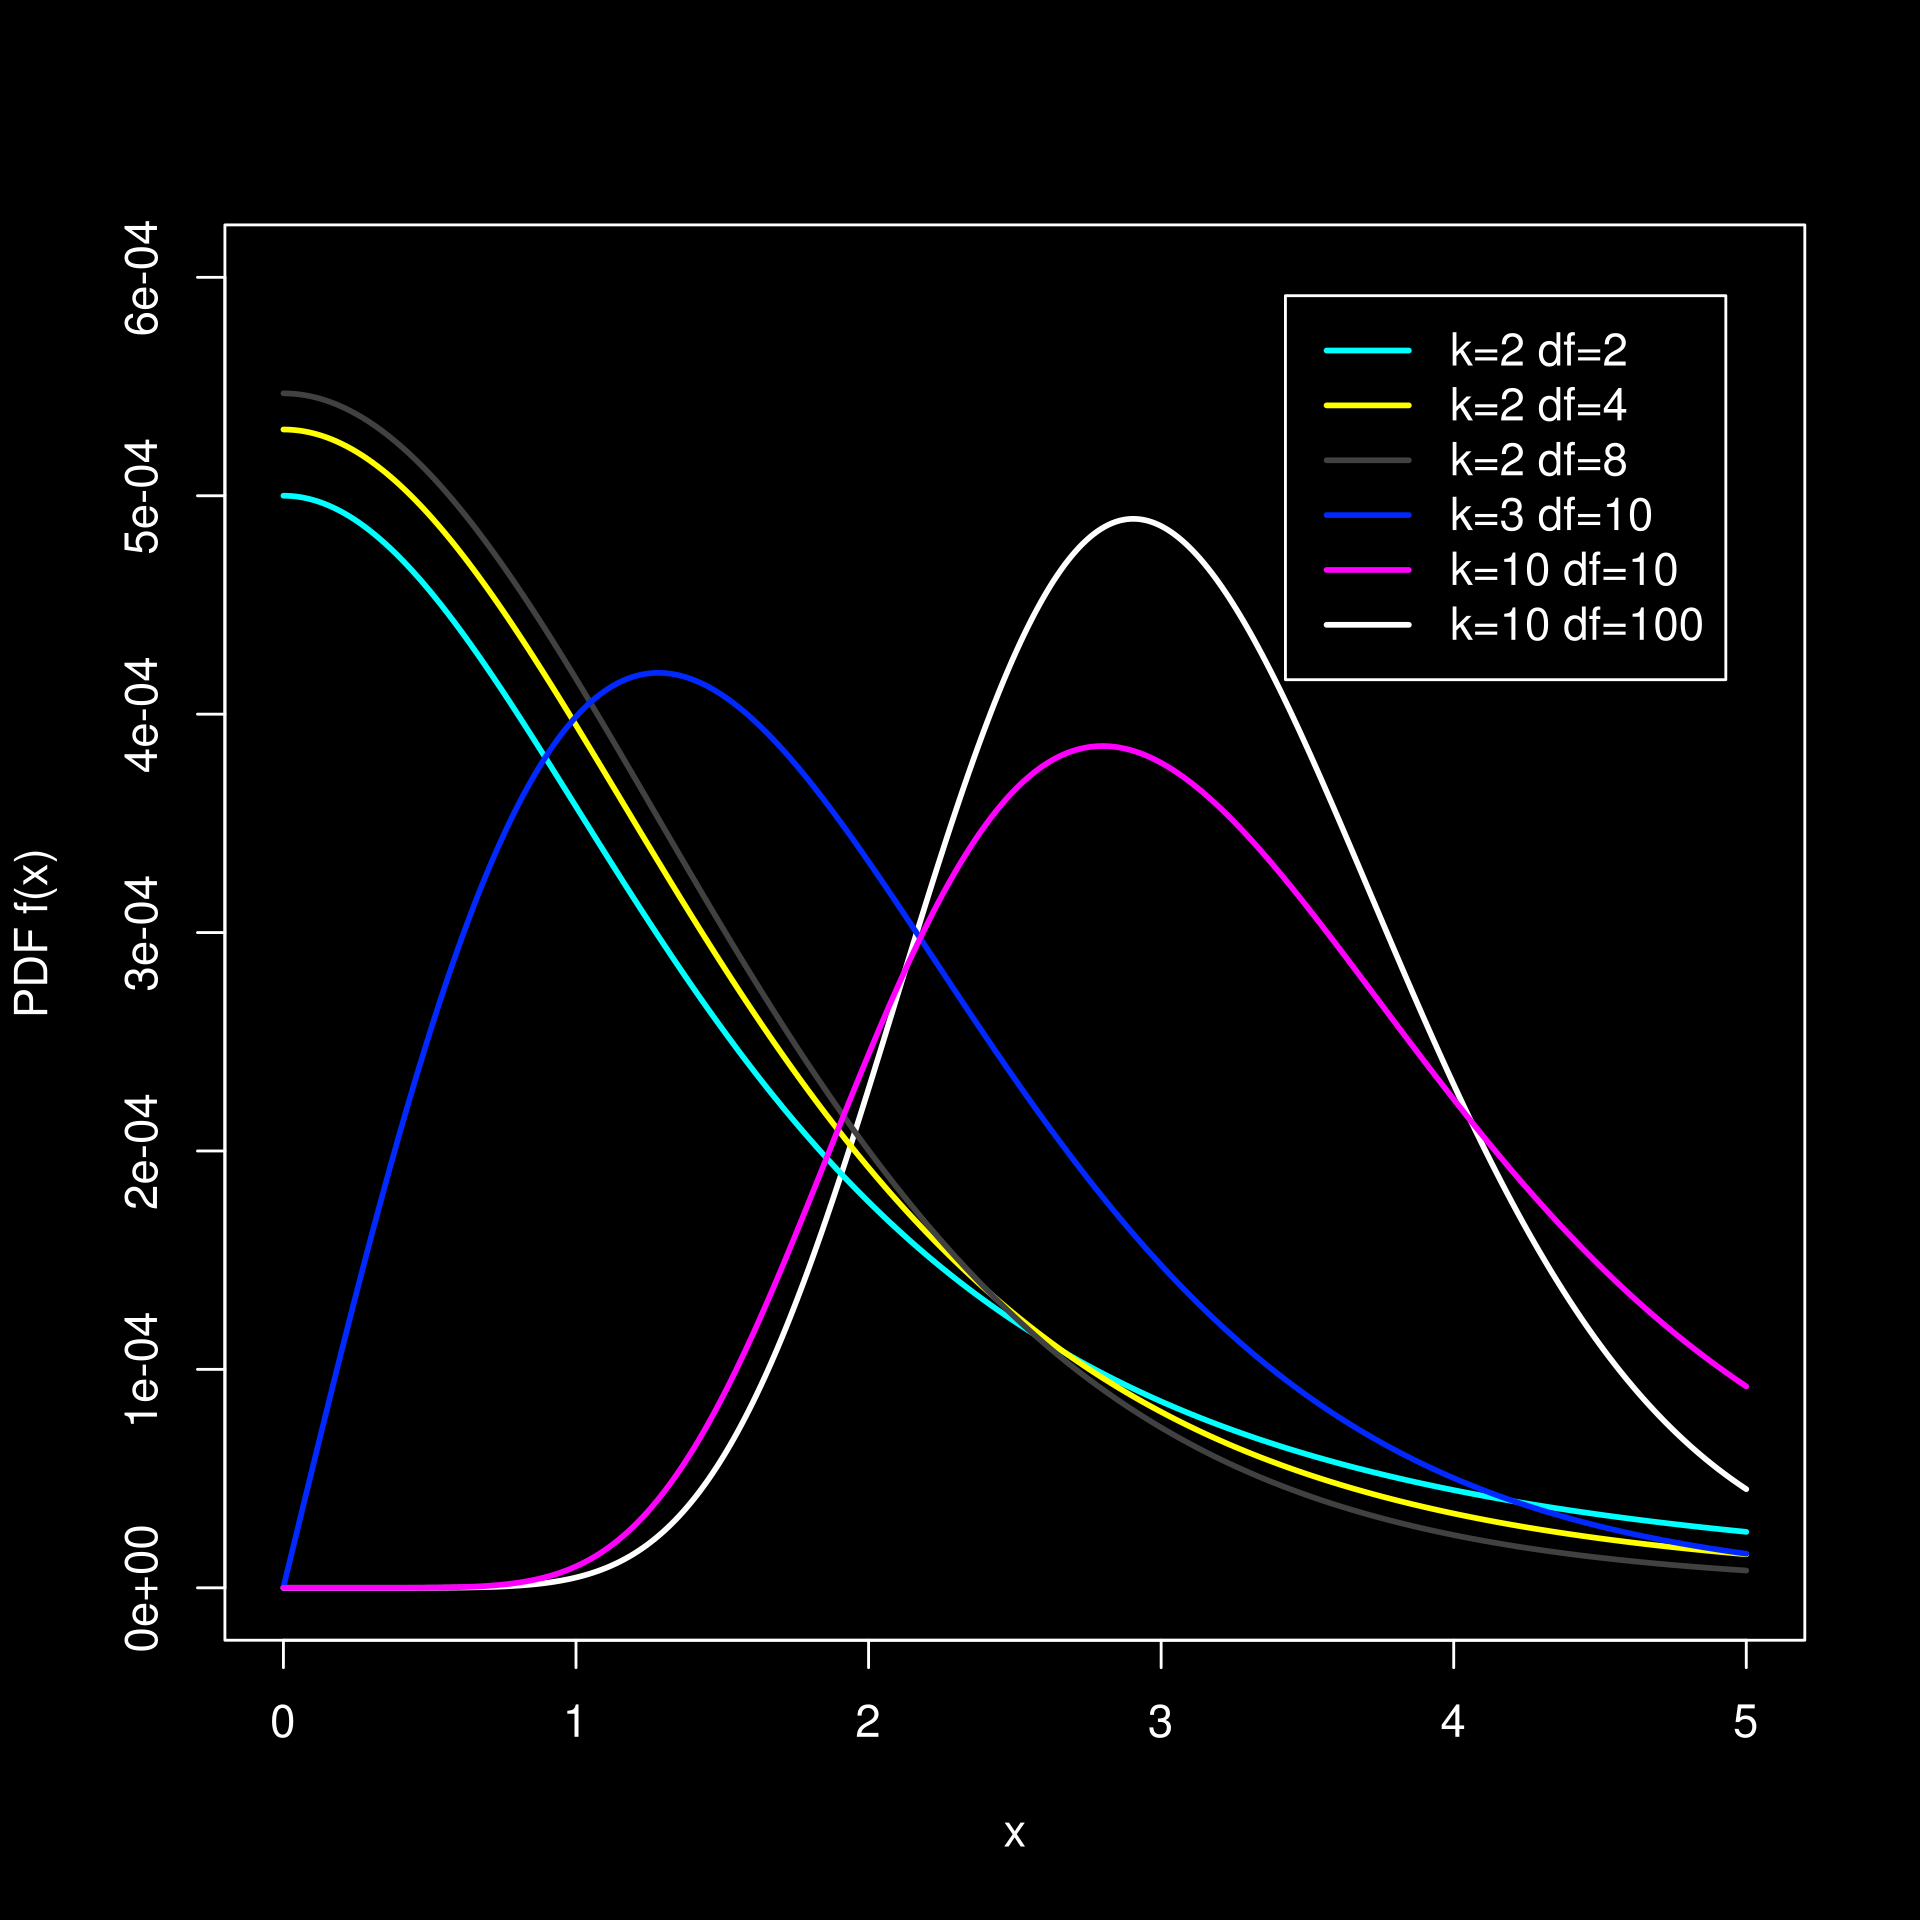
\includegraphics[scale=0.1]{1920px-StudentizedRangePDF.svg-neg.png}
	\end{center}
\end{frame}
%-------------- end slide -------------------------------%}}}
%-------------- start slide -------------------------------%{{{ 12.60
\begin{frame}[fragile]
	Let's find one example that all requirements of the $Q_{k,\nu}$ are satisfied.
	\vfill
	\begin{enumerate}
		\item Take $W_j = \overline{Y}_{\cdot j}-\mu_j$, $j=1,\cdots,k$ $\quad\Longrightarrow\quad$ $W_j\sim N(0,\sigma^2/r)$.
			\vfill
		\item $MSE$ or the pooled variance $S_p^2$ \hfill $MSE/r$
		\item[] \qquad is an unbiased estimator for $\sigma^2$ \hfill $\sigma^2/r$
		\item[] \qquad is $\perp\{\overline{Y}_{\cdot j}\}_{j=1,\cdots, k}$, hence $\perp\{W_j\}_{j=1,\cdots, k}$
			\vfill
		\item $df$ of $MSE$ is equal to $n-k=kr-k = k(r-1)$.
			\vfill
		\item[$\Longrightarrow$] \hspace{1em} $\displaystyle \frac{\max_{i}W_i - \min_j W_j}{\sqrt{MSE/r}} \sim $ Studentized range distribution($k$, $rk-k$)
	\end{enumerate}
\end{frame}
%-------------- end slide -------------------------------%}}}
%-------------- start slide -------------------------------%{{{ 12.61
\begin{frame}[fragile]

	\begin{enumerate}
		\item[]
	\[
		\hspace{3em}		\bbP \left( \frac{\max_{i}W_i - \min_j W_j}{\sqrt{MSE/r}} \le Q_{\alpha,k,rk-k}  \right ) = 1-\alpha
	\]
		\item[]
	\[||\]
	\[
		\bbP \left(\max_i W_i -\min_j W_j \le \frac{Q_{\alpha,k,rk-k}}{\sqrt{r}}\sqrt{MSE}\right)
	\]
		\item[]
	\[||\]
	\[
		\bbP \left(\left| W_i -W_j\right| \le \frac{Q_{\alpha,k,rk-k}}{\sqrt{r}}\sqrt{MSE},\:\:\forall i\ne j\right)
	\]
		\item[]
	\[||\]
	\[
		\bbP \left(\left| \left(\overline{Y}_{\cdot i} -\overline{Y}_{\cdot j}\right) - (\mu_i-\mu_j)\right| \le \frac{Q_{\alpha,k,rk-k}}{\sqrt{r}}\sqrt{MSE},\:\:\forall i\ne j\right)
	\]
		\item[]
	\[||\]
	\[
		\hspace{-2em}		\bbP \left(
			\overline{Y}_{\cdot i} -\overline{Y}_{\cdot j} - \frac{Q_{\alpha,k,rk-k}}{\sqrt{r}}\sqrt{MSE}
		\le \mu_i-\mu_j \le
			\overline{Y}_{\cdot i} -\overline{Y}_{\cdot j}+ \frac{Q_{\alpha,k,rk-k}}{\sqrt{r}}\sqrt{MSE}
		,\:\: \forall i\ne j\right )
	\]
	\end{enumerate}
\end{frame}
%-------------- end slide -------------------------------%}}}
%-------------- start slide -------------------------------%{{{ 12.62
\begin{frame}[fragile]

	\begin{enumerate}
		\item[] Therefore, for all $i\ne j$,
			the $100(1-\alpha)\%$ C.I. for $ \mu_i-\mu_j $ is \\[2em]
			\[
			\overline{Y}_{\cdot i} -\overline{Y}_{\cdot j} \pm  \frac{Q_{\alpha,k,rk-k}}{\sqrt{2}}\sqrt{MSE}\sqrt{\frac 2r}
			\]
			\vfill
		\item[] To test $H_0: \mu_i=\mu_j$ for specific $i\ne j$, reject $H_0$ in favor of $H_1:\mu_i\ne\mu_j$ if the C.I. does NOT contain $0$, at the $\alpha$ level of significance.\myEnd
			\vfill
		\item[Note:] When sample sizes are not equal, use the {\bf Tukey-Kramer method}: \\[2em]
			\[
				\overline{Y}_{\cdot i} -\overline{Y}_{\cdot j} \pm  \frac{Q_{\alpha,k,rk-k}}{\sqrt{2}}\sqrt{MSE}\sqrt{\frac{1}{r_i} + \frac{1}{r_j}}
			\]
	\end{enumerate}
\end{frame}
%-------------- end slide -------------------------------%}}}
%-------------- start slide -------------------------------%{{{ 12.63
\begin{frame}
	\begin{enumerate}
		\item[E.g. 2] A certain fraction of antibiotics injected into the bloodstream are ``bound'' to
serum proteins. This phenomenon bears directly on the effectiveness of the
medication, because the binding decreases the systemic uptake of the drug.
Table below lists the binding percentages in bovine serum measured for five
widely prescribed antibiotics. Which antibiotics have similar binding
properties, and which are different? \\[1em]
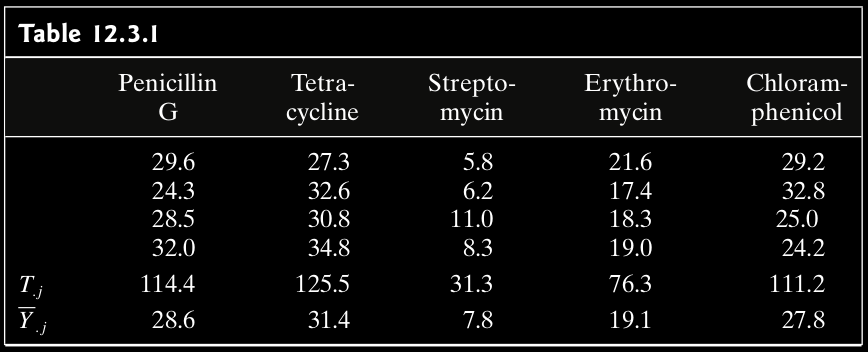
\includegraphics[scale=0.25]{Table_12-3-1-neg.png}
	\end{enumerate}
\end{frame}
%-------------- end slide -------------------------------%}}}
%-------------- start slide -------------------------------%{{{ 12.64
\begin{frame}[fragile]
	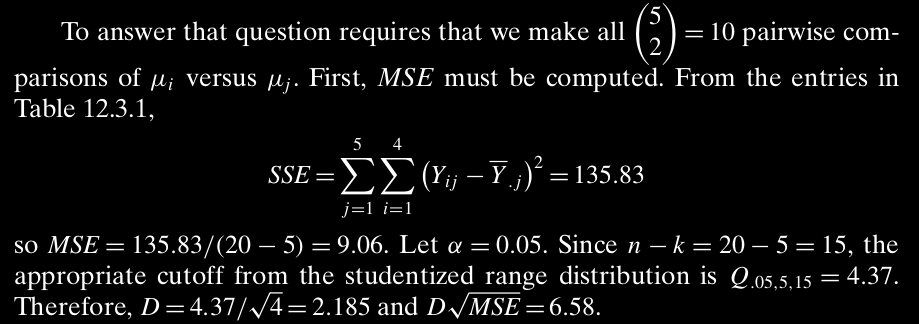
\includegraphics[scale=0.28]{Case_12-3-1-Sol1-neg.png}\\
	\vfill
	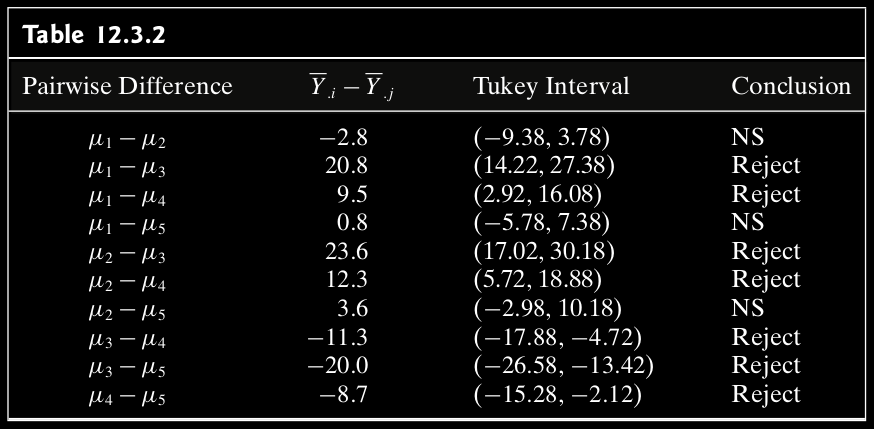
\includegraphics[scale=0.3]{Table_12-3-2-neg.png}
\end{frame}
%-------------- end slide -------------------------------%}}}
%-------------- start slide -------------------------------%{{{ 12.65
\begin{frame}[fragile]
	\begin{minipage}{0.3\textwidth}
	\begin{lstlisting}
> # Case Study 12.3.1
> # Input data first
> Input <- c("
+ rates group
+ 29.6  M1
+ 24.3  M1
+ 28.5  M1
+ 32.0  M1
+ 27.3  M2
+ 32.6  M2
+ 30.8  M2
+ 34.8  M2
+ 5.8   M3
+ 6.2   M3
+ 11.0  M3
+ 8.3   M3
+ 21.6  M4
+ 17.4  M4
+ 18.3  M4
+ 19.0  M4
+ 29.2  M5
+ 32.8  M5
+ 25.0  M5
+ 24.2 M5
+ ")
> Data = read.table(
 	textConnection(Input),
+       header=TRUE)
	\end{lstlisting}
	\end{minipage}
	\begin{minipage}{0.63\textwidth}
	\begin{lstlisting}
> # Compute one-way ANOVA test
> res.aov <- aov(rates ~ group, data = Data)
> # Summary of the analysis
> summary(res.aov)
            Df Sum Sq Mean Sq F value   Pr(>F)
group        4 1480.8   370.2   40.88 6.74e-08 ***
Residuals   15  135.8     9.1
---
Signif. codes:  0 '***' 0.001 '**' 0.01 '*' 0.05 '.' 0.1 ' ' 1
	\end{lstlisting}
	\end{minipage}

\end{frame}
%-------------- end slide -------------------------------%}}}
%-------------- start slide -------------------------------%{{{ 12.66
\begin{frame}[fragile]
	\begin{center}
		\begin{minipage}{0.6\textwidth}
	\begin{lstlisting}
> # Tukey multiple pairwise-comparisons
> TukeyHSD(res.aov)
  Tukey multiple comparisons of means
    95% family-wise confidence level

Fit: aov(formula = rates ~ group, data = Data)

$group
         diff        lwr        upr     p adj
M2-M1   2.775  -3.795401   9.345401 0.6928357
M3-M1 -20.775 -27.345401 -14.204599 0.0000006
M4-M1  -9.525 -16.095401  -2.954599 0.0034588
M5-M1  -0.800  -7.370401   5.770401 0.9952758
M3-M2 -23.550 -30.120401 -16.979599 0.0000001
M4-M2 -12.300 -18.870401  -5.729599 0.0003007
M5-M2  -3.575 -10.145401   2.995401 0.4737713
M4-M3  11.250   4.679599  17.820401 0.0007429
M5-M3  19.975  13.404599  26.545401 0.0000010
M5-M4   8.725   2.154599  15.295401 0.0071611
	\end{lstlisting}
		\end{minipage}
	\end{center}
\end{frame}
%-------------- end slide -------------------------------%}}}
%-------------- start slide -------------------------------%{{{ 12.67
\begin{frame}[fragile]
	\begin{center}
		\begin{minipage}{0.6\textwidth}
	\begin{lstlisting}
> round(TukeyHSD(res.aov)$group,2)
					diff   		 lwr		    upr		 p adj
M2-M1		   2.78		  -3.80		   9.35		  0.69
M3-M1		 -20.77		 -27.35		 -14.20		  0.00
M4-M1		  -9.52		 -16.10		  -2.95		  0.00
M5-M1		  -0.80		  -7.37		   5.77		  1.00
M3-M2		 -23.55		 -30.12		 -16.98		  0.00
M4-M2		 -12.30		 -18.87		  -5.73		  0.00
M5-M2		  -3.58		 -10.15		   3.00		  0.47
M4-M3		  11.25		   4.68		  17.82		  0.00
M5-M3		  19.97		  13.40		  26.55		  0.00
M5-M4		   8.73		   2.15		  15.30		  0.01
---
Signif. codes:  0 '***' 0.001 '**' 0.01 '*' 0.05 '.' 0.1 ' ' 1
(Adjusted p values reported -- single-step method)
	\end{lstlisting}
		\end{minipage}
		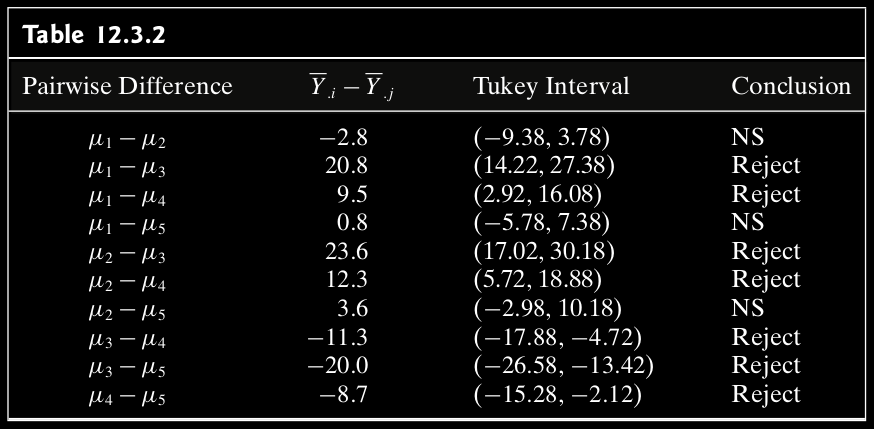
\includegraphics[scale=0.25]{Table_12-3-2-neg.png}
	\end{center}
\end{frame}
%-------------- end slide -------------------------------%}}}
%-------------- start slide -------------------------------%{{{ 12.68
\begin{frame}[fragile]
	\begin{center}
		\begin{minipage}{0.7\textwidth}
	\begin{lstlisting}
	> # Or one may use multcomp package or multiple comparisons
> library(multcomp)
> summary(glht(res.aov, linfct = mcp(group = "Tukey")))

	 Simultaneous Tests for General Linear Hypotheses

Multiple Comparisons of Means: Tukey Contrasts


Fit: aov(formula = rates ~ group, data = Data)

Linear Hypotheses:
             Estimate Std. Error t value Pr(>|t|)
M2 - M1 == 0    2.775      2.128   1.304  0.69283
M3 - M1 == 0  -20.775      2.128  -9.764  < 0.001 ***
M4 - M1 == 0   -9.525      2.128  -4.477  0.00348 **
M5 - M1 == 0   -0.800      2.128  -0.376  0.99528
M3 - M2 == 0  -23.550      2.128 -11.068  < 0.001 ***
M4 - M2 == 0  -12.300      2.128  -5.781  < 0.001 ***
M5 - M2 == 0   -3.575      2.128  -1.680  0.47374
M4 - M3 == 0   11.250      2.128   5.287  < 0.001 ***
M5 - M3 == 0   19.975      2.128   9.388  < 0.001 ***
M5 - M4 == 0    8.725      2.128   4.101  0.00717 **
---
Signif. codes:  0 '***' 0.001 '**' 0.01 '*' 0.05 '.' 0.1 ' ' 1
(Adjusted p values reported -- single-step method)
	\end{lstlisting}
		\end{minipage}
	\end{center}
\end{frame}
%-------------- end slide -------------------------------%}}}
%-------------- start slide -------------------------------%{{{ 12.69
\begin{frame}[fragile]
	\begin{center}
		\begin{minipage}{0.7\textwidth}
	\begin{lstlisting}
	             Estimate Std. Error t value Pr(>|t|)
M2 - M1 == 0    2.775      2.128   1.304  0.69283
M3 - M1 == 0  -20.775      2.128  -9.764  < 0.001 ***
M4 - M1 == 0   -9.525      2.128  -4.477  0.00348 **
M5 - M1 == 0   -0.800      2.128  -0.376  0.99527
M3 - M2 == 0  -23.550      2.128 -11.068  < 0.001 ***
M4 - M2 == 0  -12.300      2.128  -5.781  < 0.001 ***
M5 - M2 == 0   -3.575      2.128  -1.680  0.47371
M4 - M3 == 0   11.250      2.128   5.287  < 0.001 ***
M5 - M3 == 0   19.975      2.128   9.388  < 0.001 ***
M5 - M4 == 0    8.725      2.128   4.101  0.00719 **
	\end{lstlisting}
		\end{minipage}
		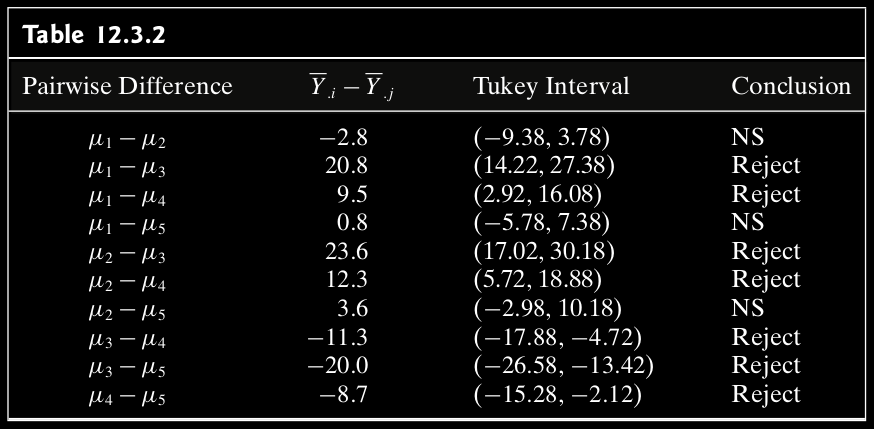
\includegraphics[scale=0.25]{Table_12-3-2-neg.png}
	\end{center}
\end{frame}
%-------------- end slide -------------------------------%}}}
%-------------- start slide -------------------------------%{{{ 12.70
\begin{frame}{Two more examples of ANOVA using R}
	\begin{enumerate}
		\item[E.g. 1] \url{http://www.sthda.com/english/wiki/one-way-anova-test-in-r}
			\vfill
		\item[E.g. 2] \url{https://datascienceplus.com/one-way-anova-in-r/}
	\end{enumerate}
\end{frame}
%-------------- end slide -------------------------------%}}}

% \mySection{12.4 Testing Subhypotheses with Contrasts}
%-------------- start slide -------------------------------%{{{ 12.73
\begin{frame}
		% {\S\: 12.4 Testing Subhypotheses with Contrasts}
\end{frame}
%-------------- end slide -------------------------------%}}}

\end{document}

